\subsection{Kompressionsverfahren: Diskrete Kosinus Transformation} \label{resultate:loesung1}
In diesem Abschnitt wird die Kompression mittels Diskreter Kosinus Transformation behandelt. Es wurden verschiedene Transformationen getestet, welche die Approximation mittels Kosinus Funktionen verbessern. Die Ableitung der Feldlinien dämpft die Kompressionsartefakte und ist massgebend für die Kompressionsrate verantwortlich.\\
Um die Feldlinien optimal mit der DCT zu approximieren, müssen Ringing-Artefakte, behandelt werden. Das Auftreten der Artefakte wird im Abschnitt \ref{resultate:loesung1:ringing} und die Behandlung im Abschnitt \ref{resultate:loesung1:behandlung_ringing} besprochen.

\subsubsection{Variante: DCT}\label{resultate:dct}

\begin{figure}[!htbp]
	\center
	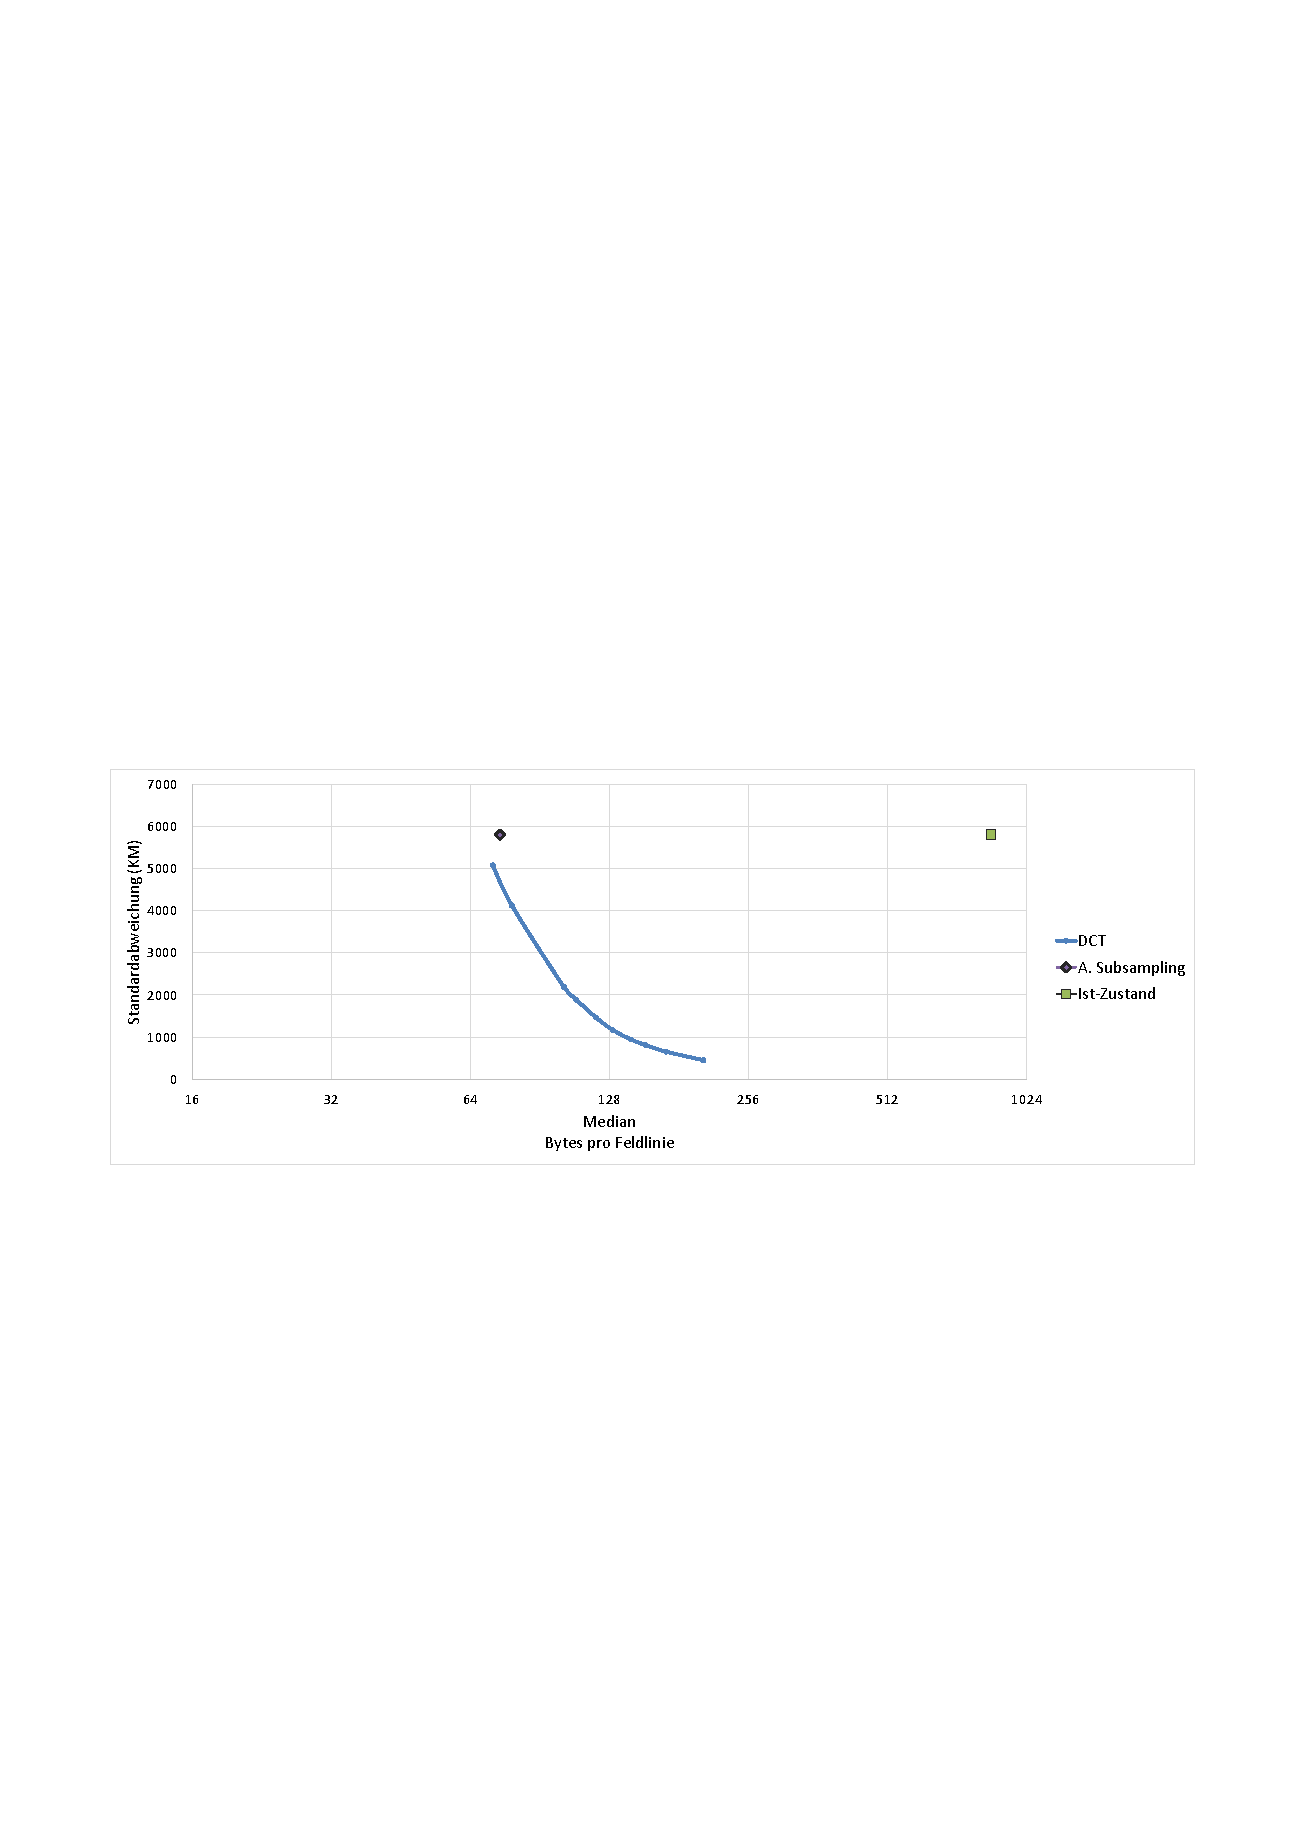
\includegraphics[trim = 1.8cm 11.5cm 1.8cm 13cm, clip=true,width=1\textwidth,keepaspectratio]{./pictures/resultate/loesung1/loesung1-0/loesung1_0.pdf}
	\caption{Vergleich der DCT Kompression mit dem Verfahren des Adaptiven Subsamplings}
	\label{resultate:loesung1:dct:resultate}
\end{figure}
Die Abbildung \ref{resultate:loesung1:dct:resultate} zeigt den Vergleich der DCT Kompression mit dem Verfahren des Adaptiven Subsamplings (siehe \ref{resultate:loesung0}). Die Standardabweichung steigt mit stärkerer Quantisierung unerwartet schnell an. Der Grund dafür kann im Diagramm der Abbildung \ref{resultate:loesung1:dct:artefakte} entnommen werden:

\begin{figure}[!htbp]
	\center
	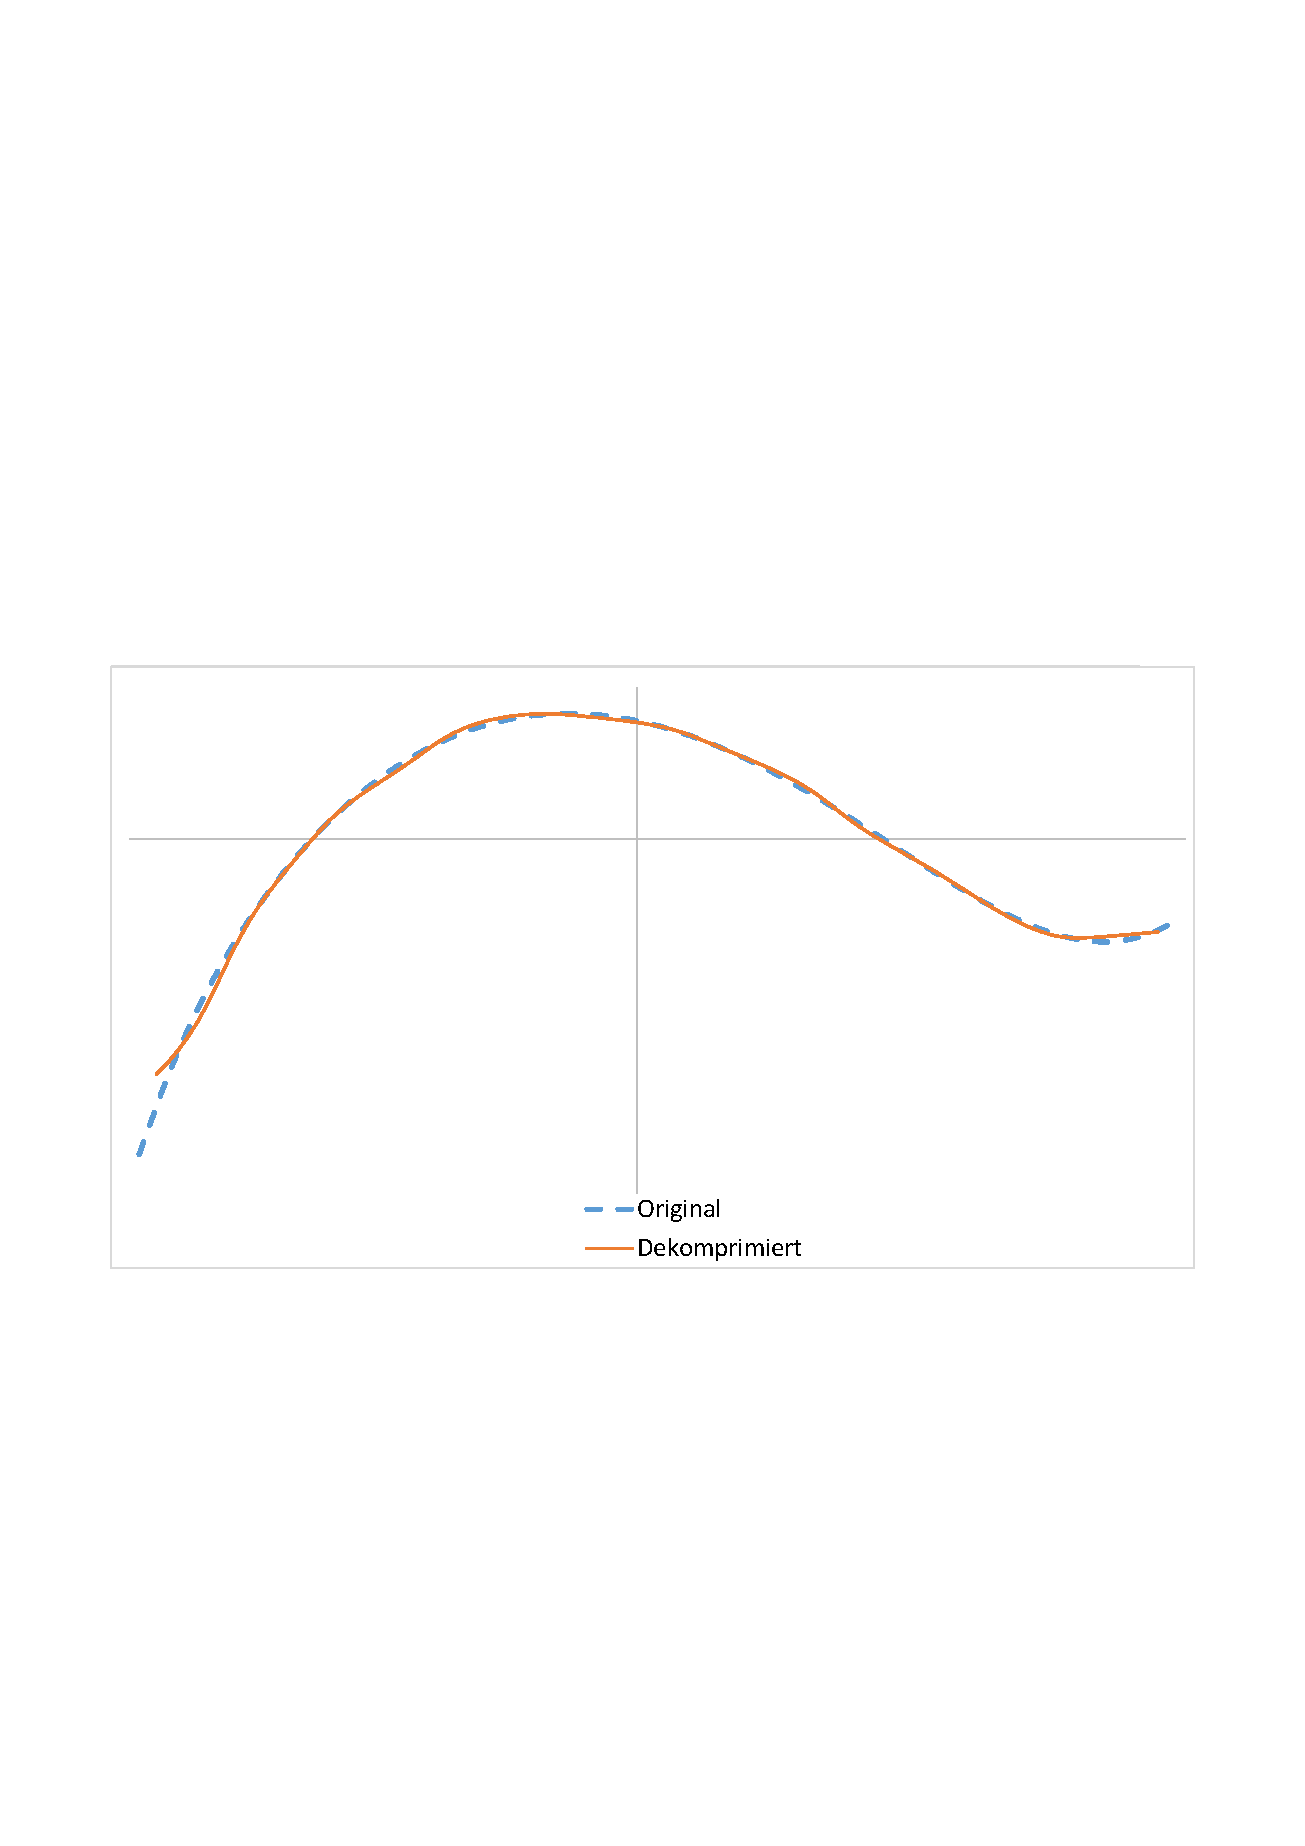
\includegraphics[trim = 1.8cm 9.8cm 1.8cm 11.2cm, clip=true, width=0.8\textwidth,height=8cm,keepaspectratio]{./pictures/resultate/loesung1/loesung1-0/loesung1_0_artefakte.pdf}
	\caption{Artefakte der DCT Dekompression anhand Beispieldaten}
	\label{resultate:loesung1:dct:artefakte}
\end{figure}
Der Anfang und das Ende der Feldlinie können nicht gut approximiert werden. Dies ist ein typisches Problem der DCT: Ein Inputsignal wird in der DCT konzeptionell repetiert, da die DCT nur ein periodisches Signal transformieren kann. Dazu wird konzeptionell das Signal gespiegelt. Das Diagramm der Abbildung \ref{resultate:loesung1:dct:spiegelung} illustriert das Problem. Bei der Beispielfeldlinie aus Abbildung \ref{resultate:loesung1:dct:artefakte} führt die Wiederholung zu einer Spitze im Signal. Die Spitze wird in der DCT mit hochfrequenten Anteilen abgebildet, welche von der Quantisierung gelöscht werden. Das Ergebnis ist eine Verschiebung an den Stellen, wo die Spitze auftritt. In diesem Fall ist es jeweils am Anfang und am Ende der Feldlinie.

\begin{figure}[!htbp]
	\center
	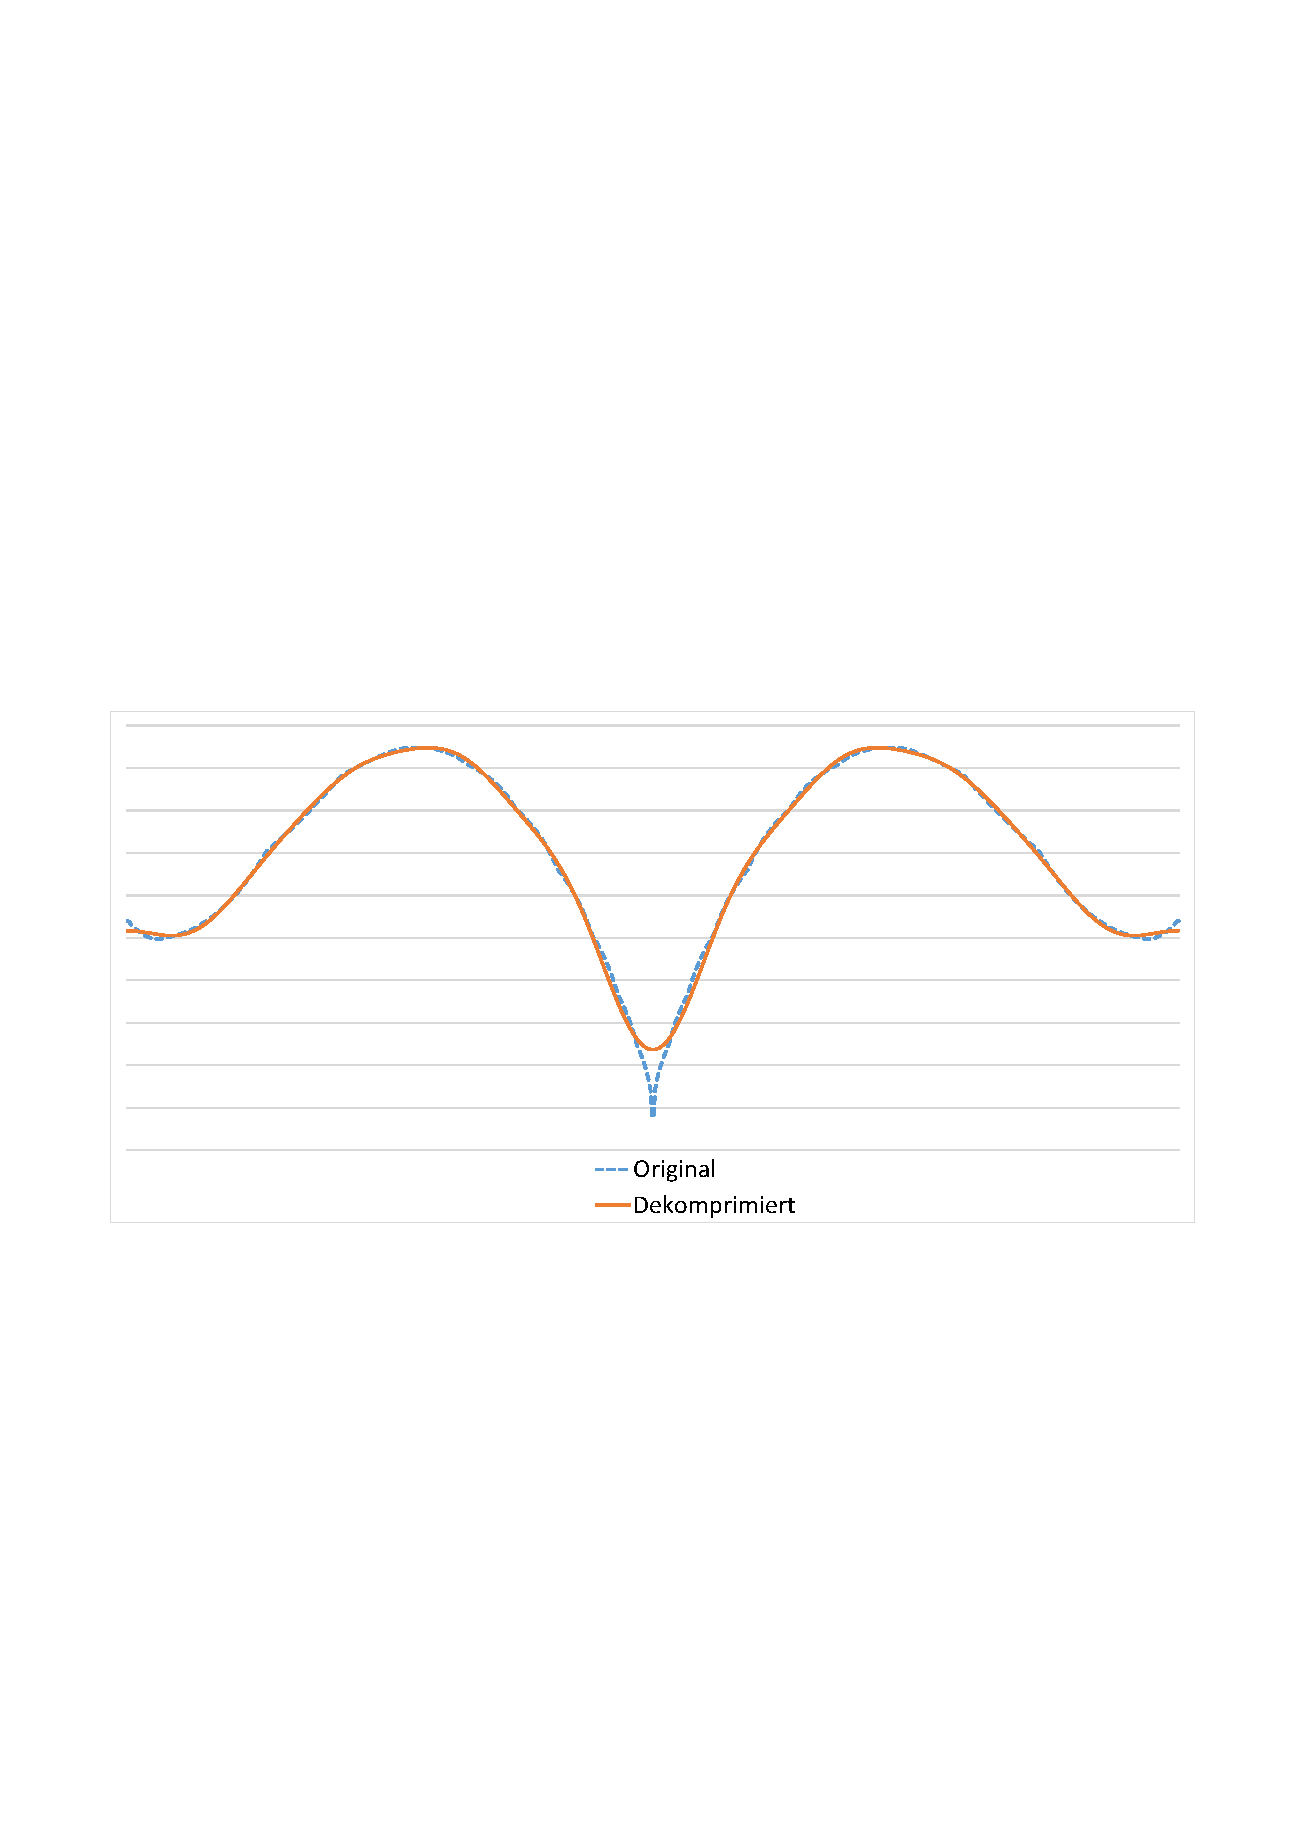
\includegraphics[trim = 1.8cm 10.5cm 1.8cm 12cm, clip=true, width=0.8\textwidth,height=8cm,keepaspectratio]{./pictures/resultate/loesung1/loesung1-0/spiegelung.pdf}
	\caption{Konzeptionelle Spiegelung an den Rändern des Signals.}
	\label{resultate:loesung1:dct:spiegelung}
\end{figure}
Das Problem kann entweder durch eine vorhergehende Transformation der Feldlinie oder durch zusätzliche Daten am Anfang und am Ende der Linie gelöst werden. Die Variante, welche die Feldlinie mit Daten erweitert, wird im Abschnitt \ref{resultate:loesung1:dct:randbeh+byte} behandelt. Eine andere Darstellung der Feldlinie wird in den folgenden Abschnitten behandelt.

\subsubsection{Variante: Ableitung+DCT}\label{resultate:dct:ableitung_dct}
Vor der Diskreten Kosinus Transformation werden die Feldlinien abgeleitet. Durch diese Darstellung werden die Artefakte aus der Abbildung \ref{resultate:loesung1:dct:artefakte} behoben.

\begin{figure}[!htbp]
	\center
	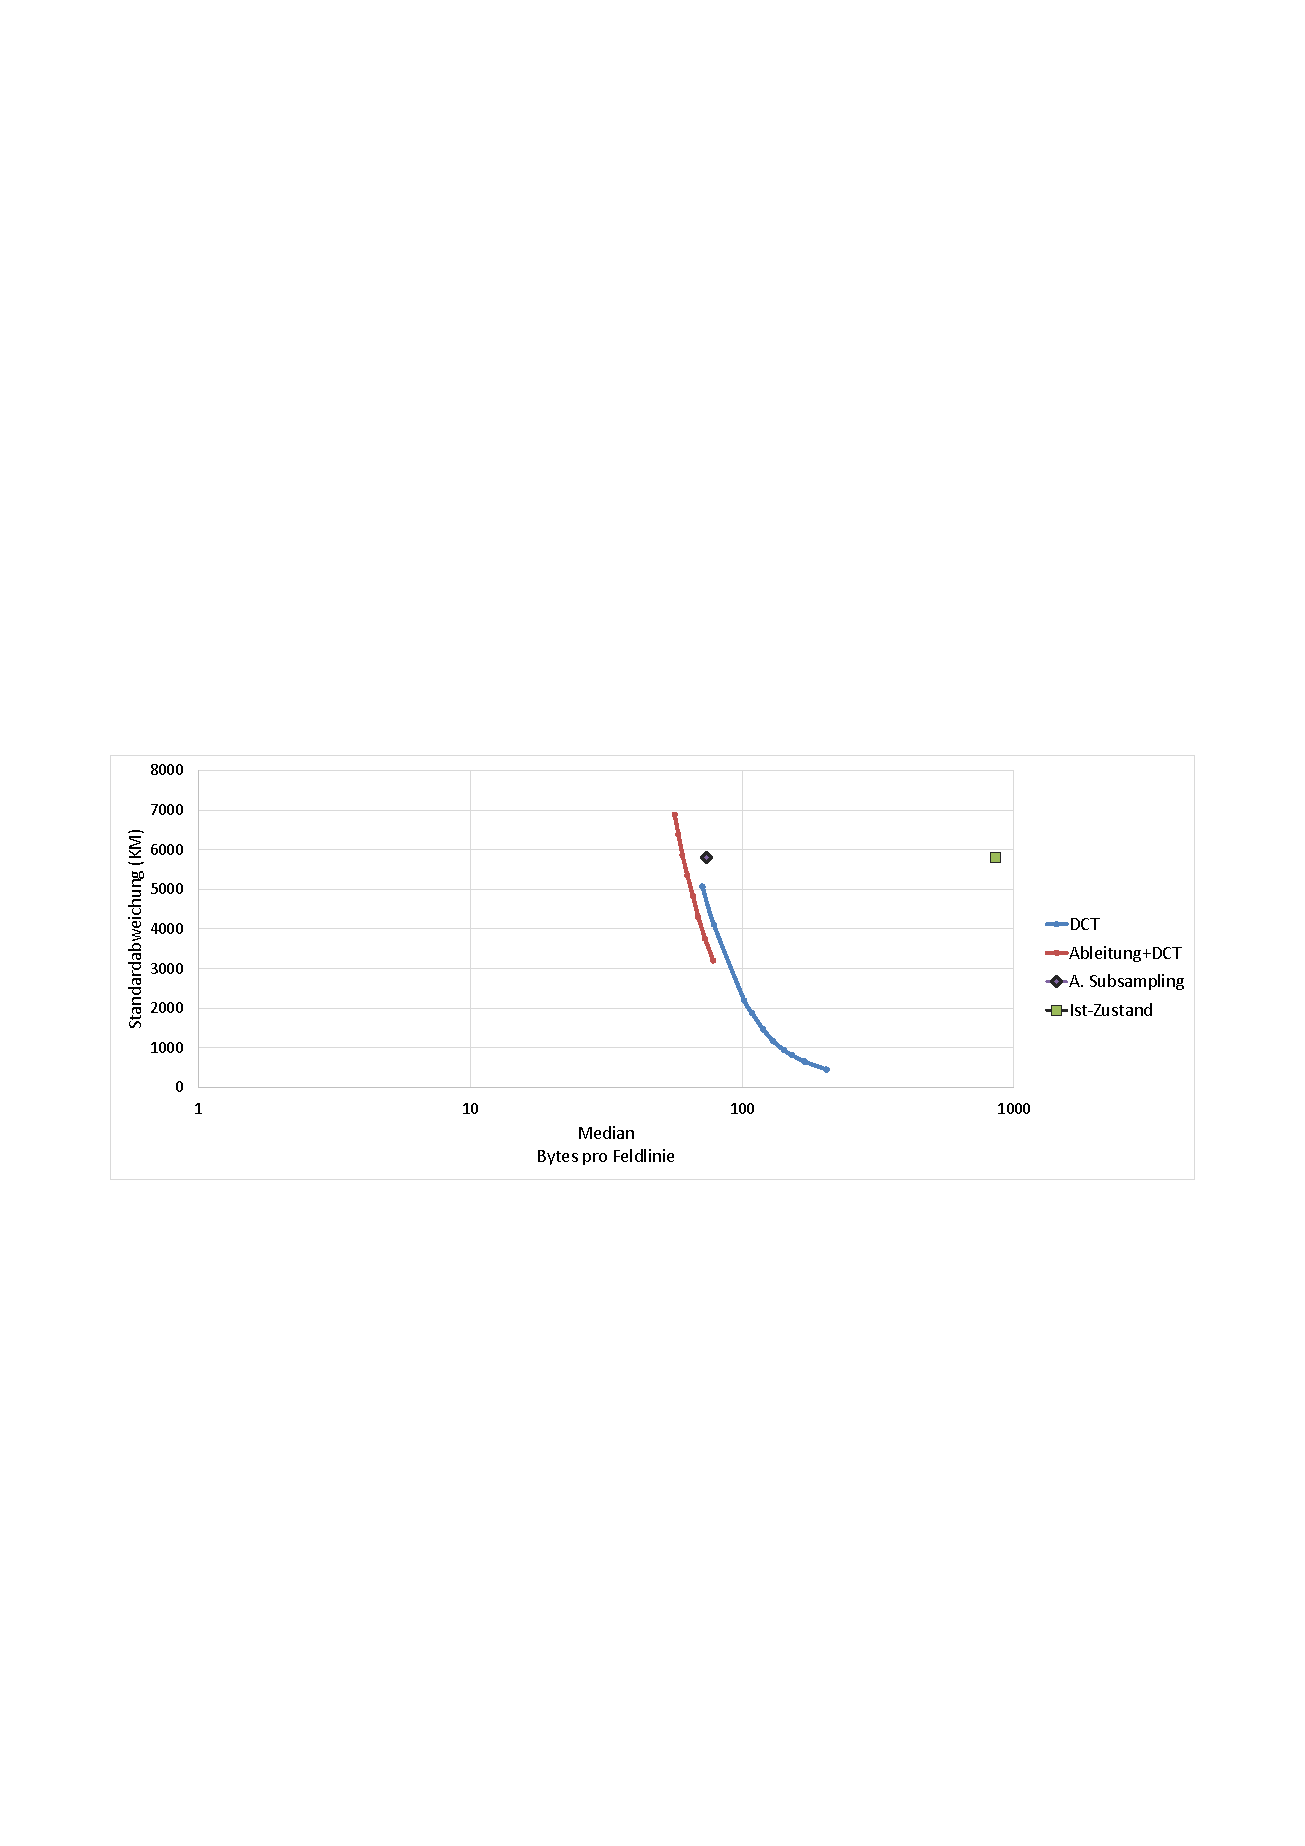
\includegraphics[trim = 1.8cm 11.25cm 1.8cm 12.75cm, clip=true, width=1\textwidth,keepaspectratio]{./pictures/resultate/loesung1/loesung1-1/resultate_loesung1_1.pdf}
	\caption{Vergleich der DCT Kompression der Ableitung mit der DCT Kompression}
	\label{resultate:loesung1:dct_ableitung:resultate}
\end{figure}
Das Diagramm der Abbildung \ref{resultate:loesung1:dct_ableitung:resultate} zeigt, dass die abgeleiteten Feldlinien besser approximiert werden können als die vorhergehende Variante. Bei einer vergleichbaren Genauigkeit wie der Ist-Zustand erreicht diese Variante eine Kompressionsrate von 14.3. Eine Darstellung der Artefakte ist im Diagramm der Abbildung \ref{resultate:loesung1:dct:byte:artefakte} zu finden. Die Artefakte der Kompression äussern sich als Dämpfungen. Die Artefakte sind jedoch für das menschliche Auge nicht sichtbar. Die Dämpfung ist erst zu erkennen, wenn das Original zur Verfügung steht.

\begin{figure}[!htbp]
	\center
	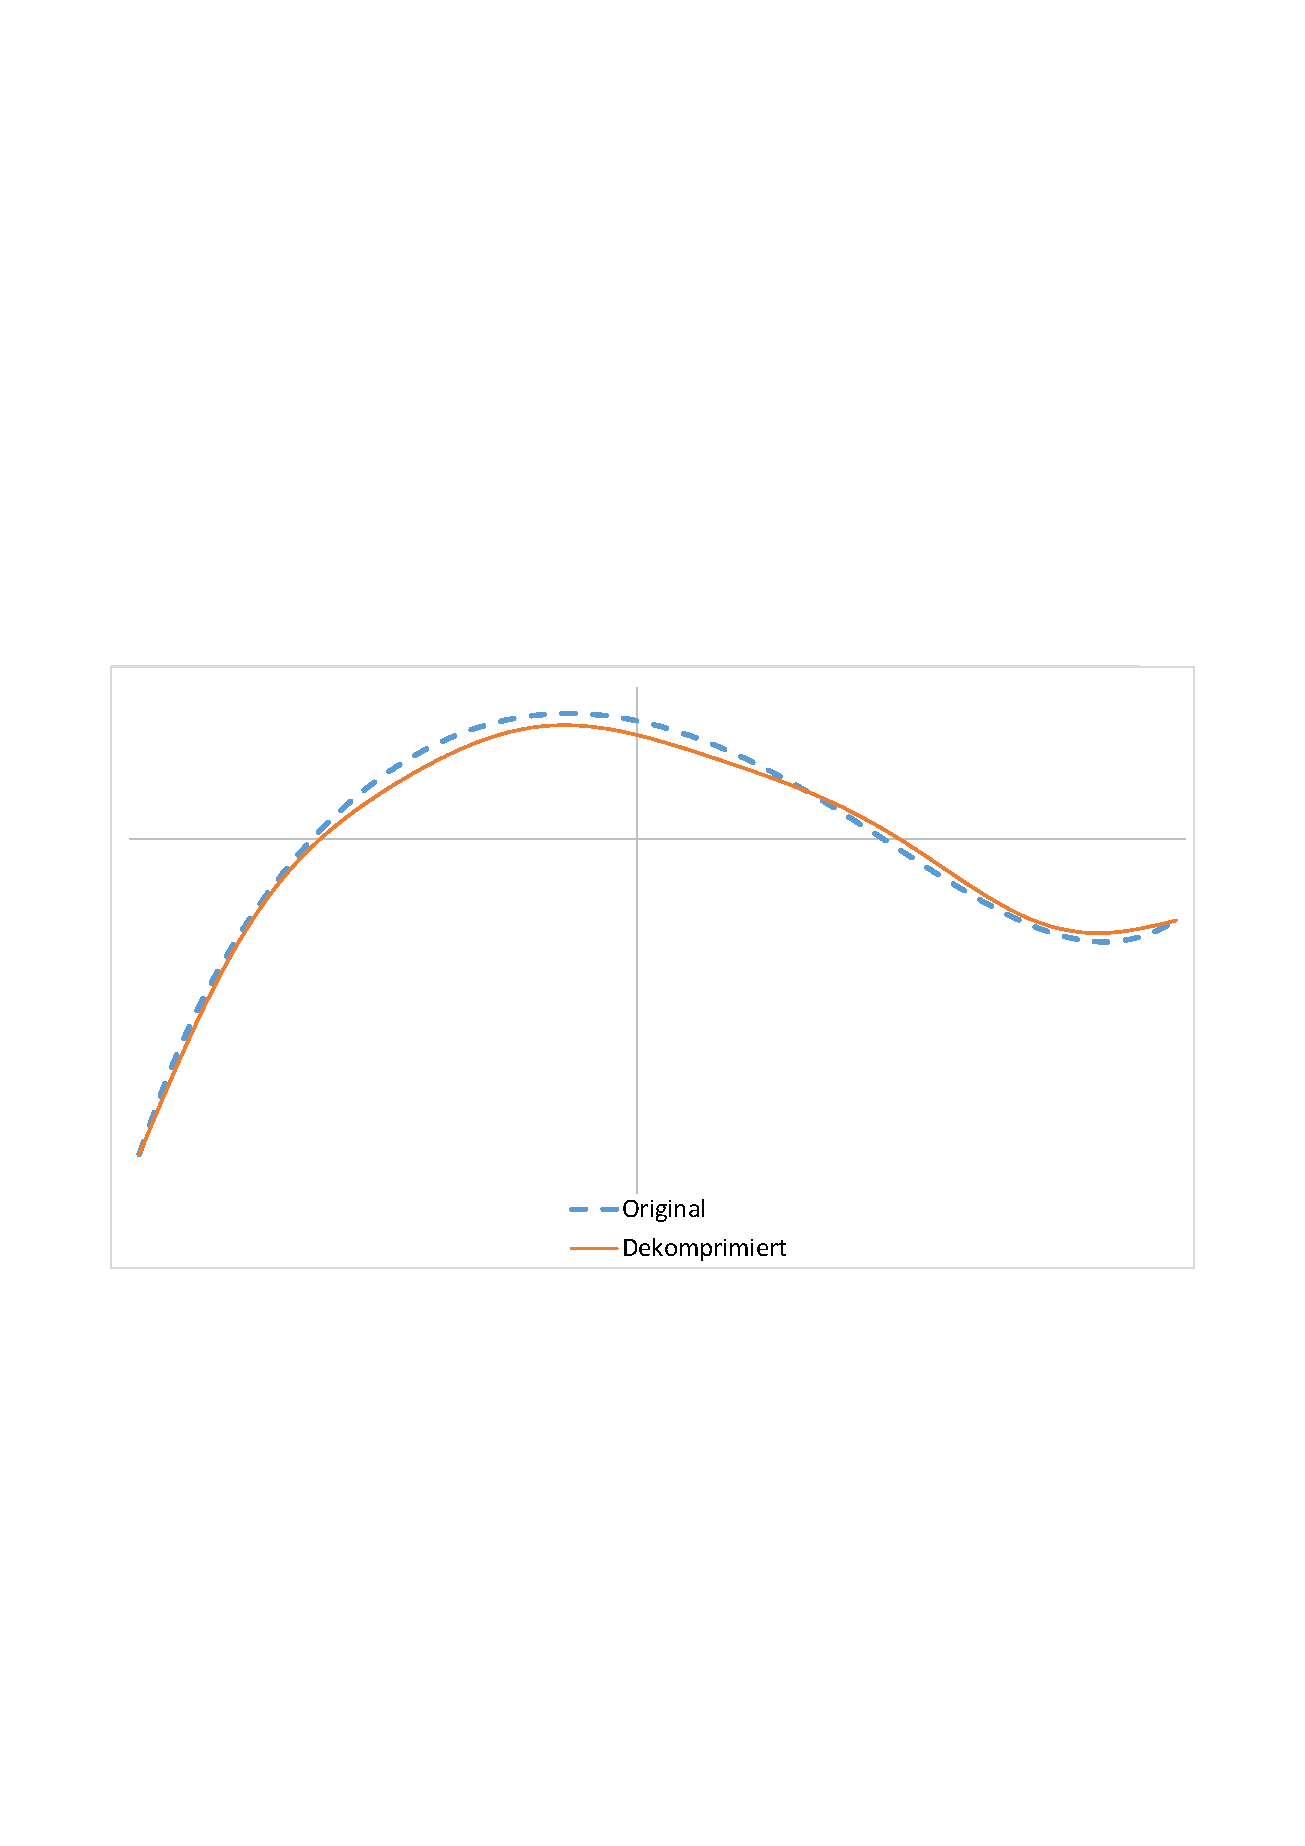
\includegraphics[trim = 1.8cm 9.5cm 1.8cm 11cm, clip=true,width=0.8\textwidth,height=8cm,keepaspectratio]{./pictures/resultate/loesung1/loesung1-6/artefakte.pdf}
	\caption{Artefakte der DCT Kompression der Ableitung}
	\label{resultate:loesung1:dct:byte:artefakte}
\end{figure} 

\subsubsection{Variante: PCA+Ableitung+DCT}
Durch eine Principal Component Analysis (PCA) \cite{abdi2010principal} können die Feldlinien in ein lokales Koordinatensystem transformiert werden. Die PCA legt die Koordinatenachsen entlang der höchsten Varianz der Daten. Das bedeutet, dass entlang der ersten Achse der höchste Informationsanteil der Feldlinie zu finden ist, entlang der zweiten Achse die zweithöchste etc. Die Achsen werden unterschiedlich stark quantisiert. Für die Rücktransformation ins Sonnen-Koordinatensystem werden pro Feldlinie zusätzlich sechs Parameter für die neuen Koordinatenachsen und drei Parameter für die Verschiebung abgespeichert.

\begin{figure}[!htbp]
	\center
	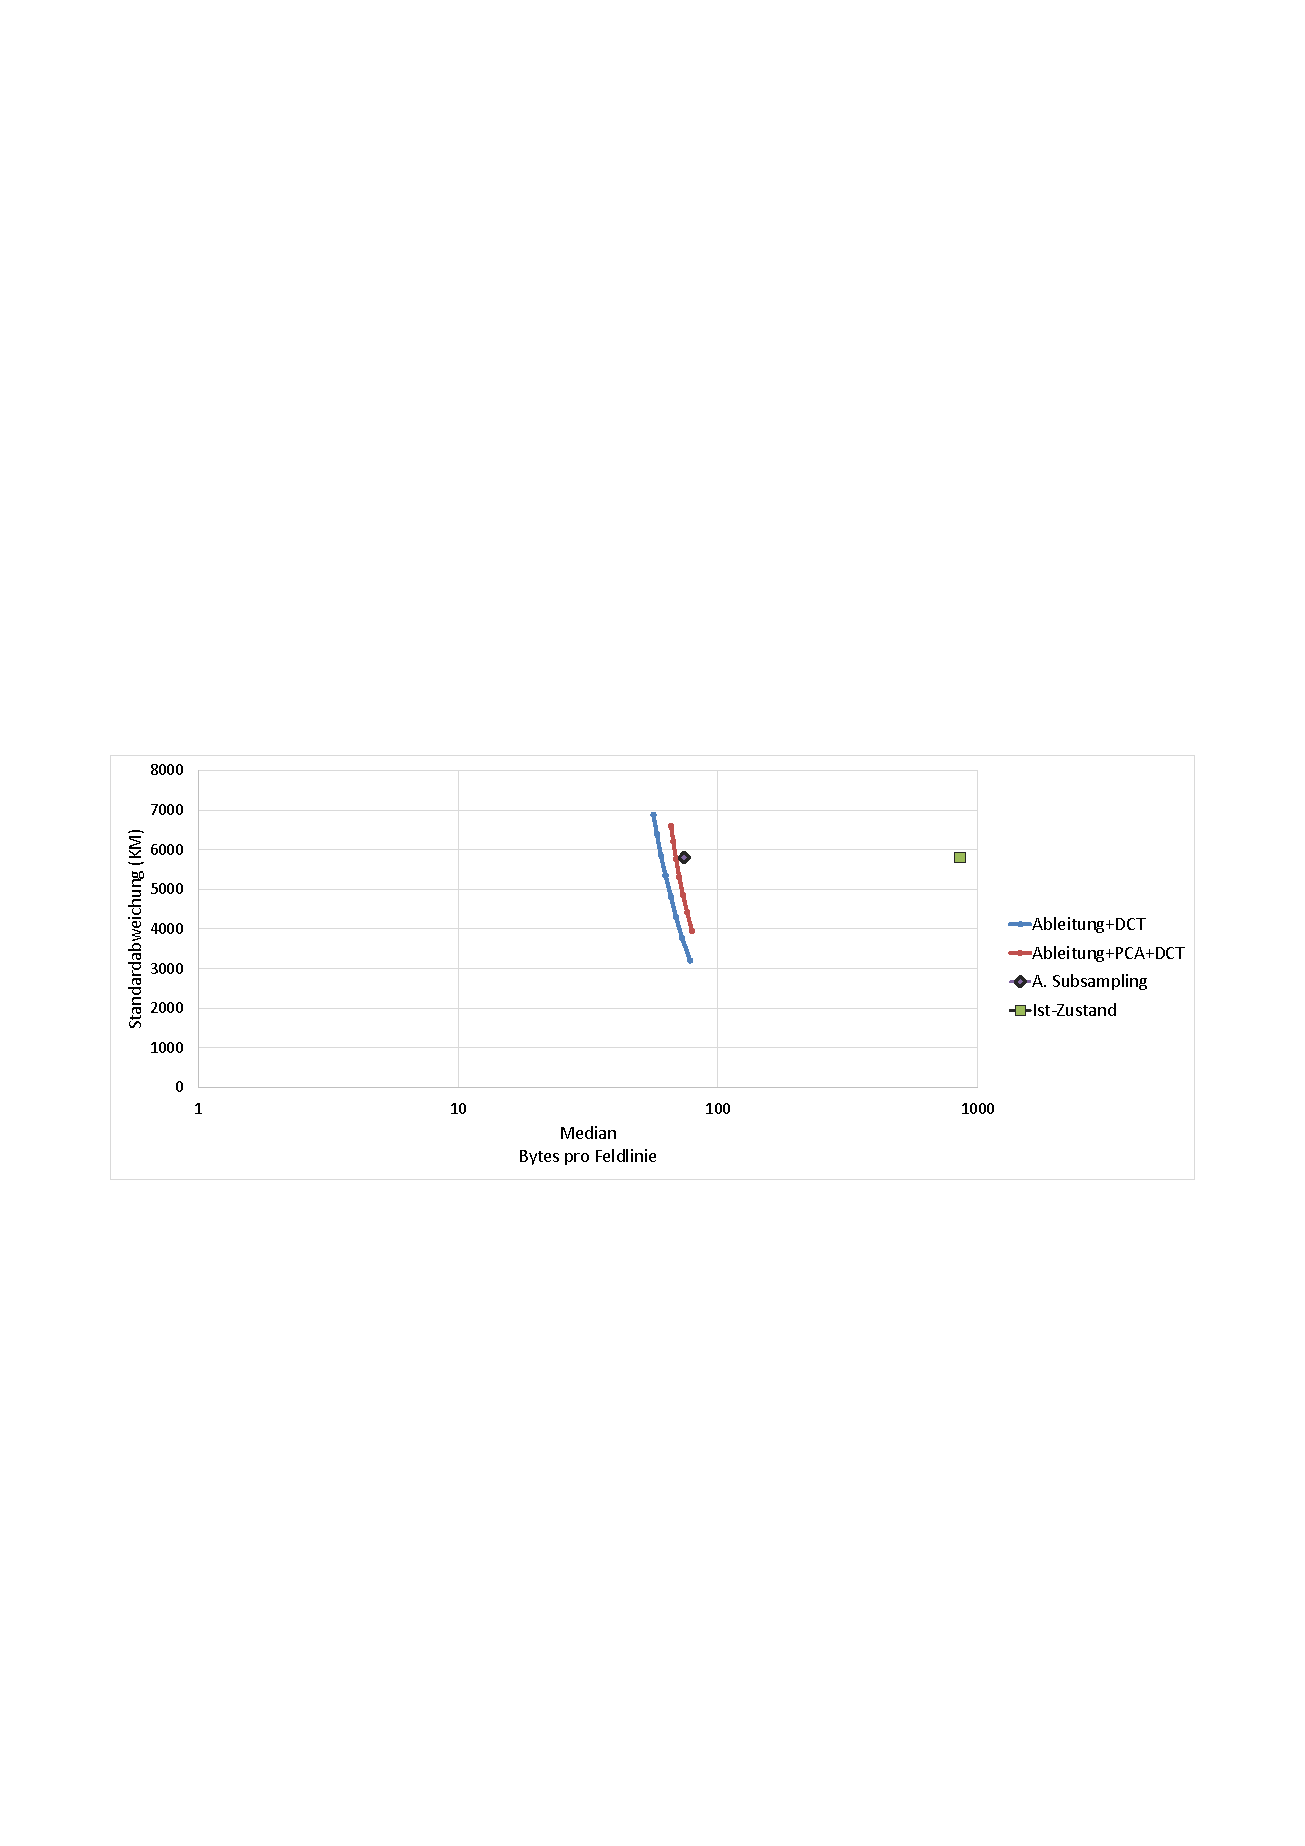
\includegraphics[trim = 1.8cm 11.25cm 1.8cm 12.75cm, clip=true,width=1\textwidth,keepaspectratio]{./pictures/resultate/loesung1/loesung1-4/loesung1_4.pdf}
	\caption{Vergleich der PCA DCT Kompression der Ableitung mit der DCT Kompression der Ableitung}
	\label{resultate:loesung1:dct:pca}
\end{figure}
Im Diagramm der Abbildung \ref{resultate:loesung1:dct:pca} sind die Resultate der Messung dargestellt. Die PCA konnte keine Verbesserung erbringen. Für die Übermittlung der zusätzlichen Parameter wird mehr Speicherplatz benötigt, als dank der PCA gewonnen werden kann.

\subsubsection{Variante: Ableitung+DCT+Kodierung} \label{resultate:loesung1:ableitung_dct_kodierung}
Im Diagramm der Abbildung \ref{resultate:loesung1:dct:histogramm} ist zu sehen, dass der Grossteil der quantisierten DCT-Koeffizienten mit 8 Bit Genauigkeit dargestellt werden können. Um die Kompressionsrate durch diese Eigenschaft zu verbessern, wurde die Längenkodierung und die adaptive Genauigkeits-Kodierung entwickelt, welche im Abschnitt \ref{konzept:loesung1:kodierung} beschrieben sind.
\begin{figure}[!htbp]
	\center
	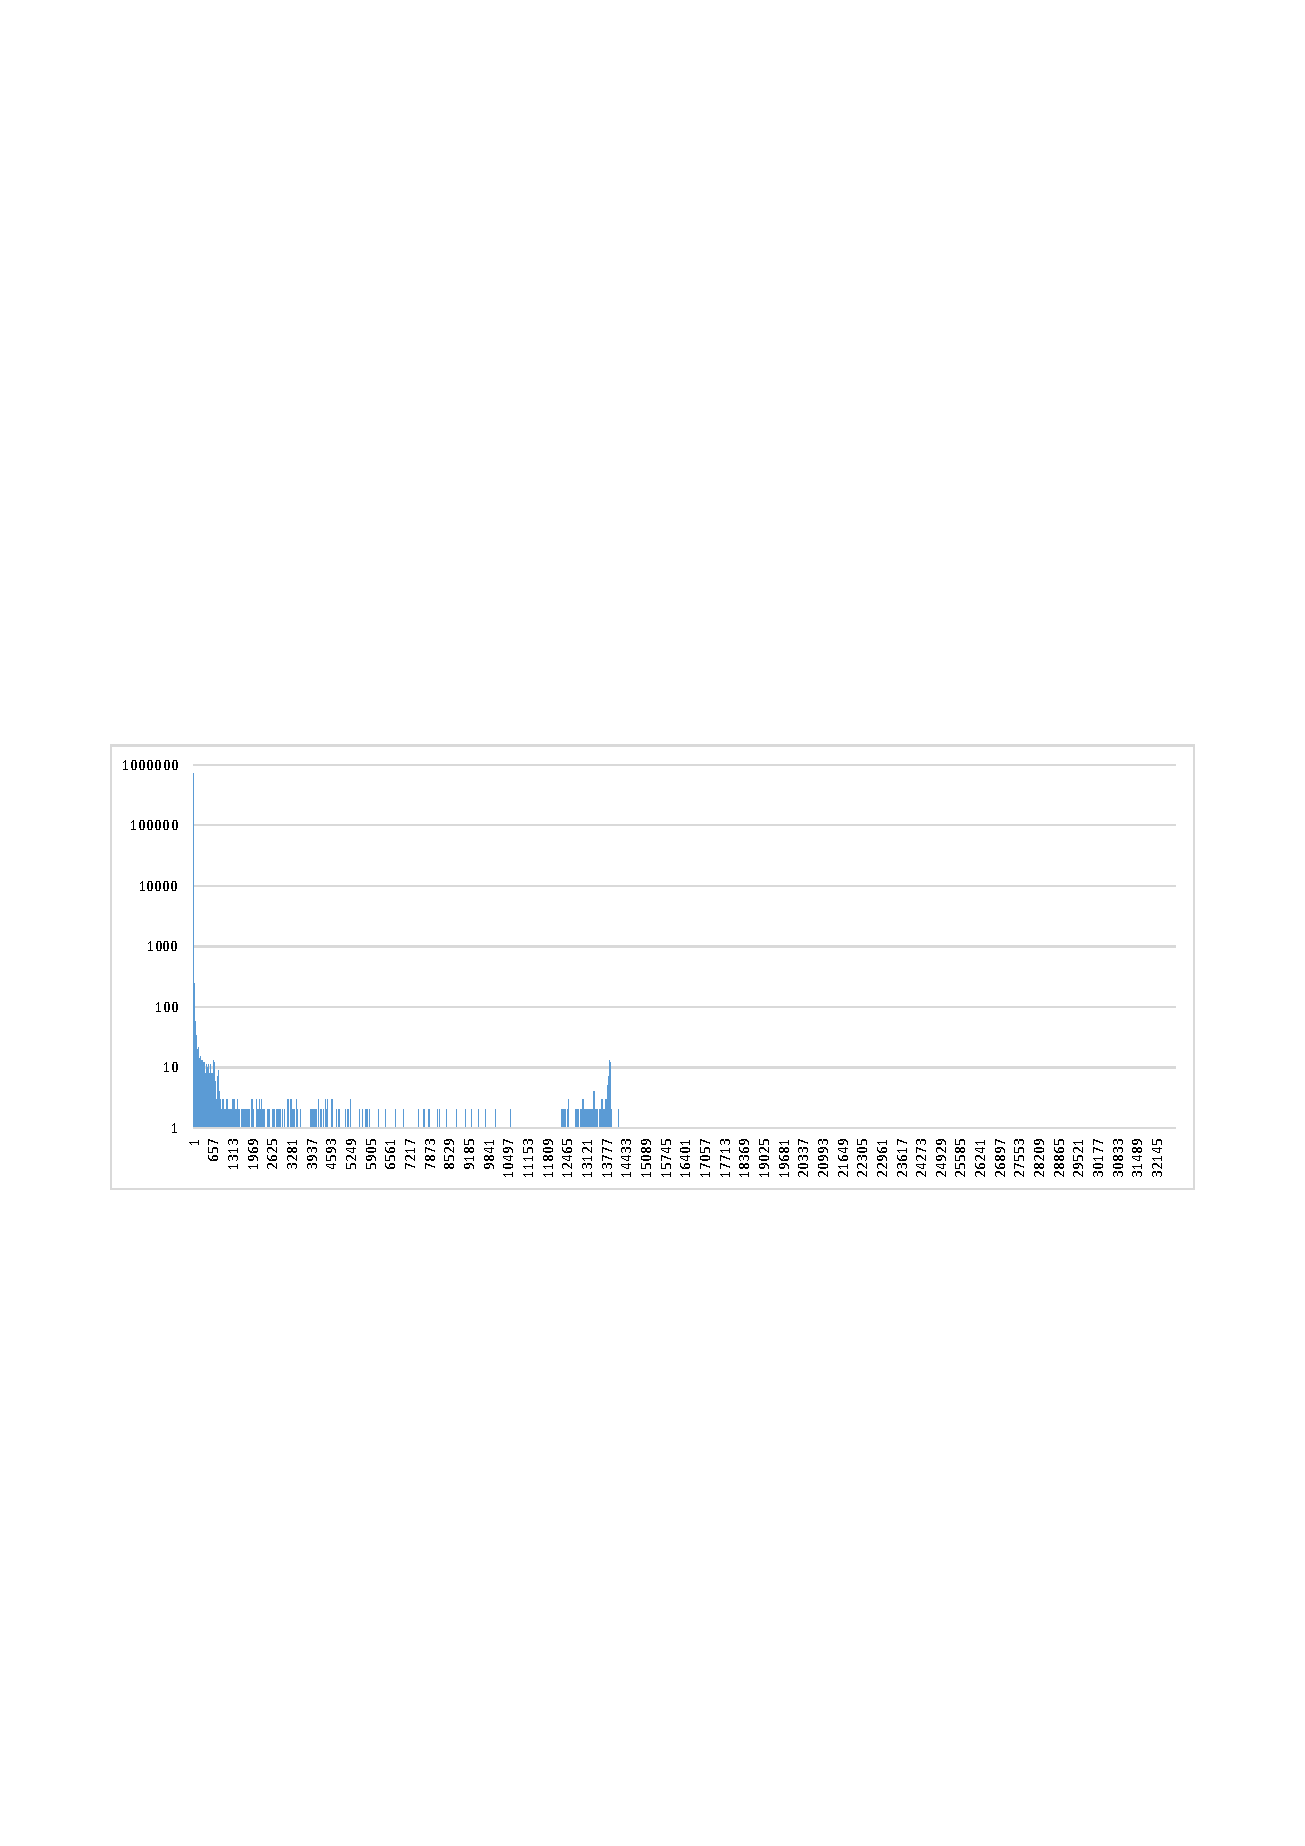
\includegraphics[trim = 1.8cm 11.25cm 1.8cm 12.75cm, clip=true,width=1\textwidth,keepaspectratio]{./pictures/resultate/loesung1/loesung1-6/histo.pdf}
	\caption{Histogramm der absoluten Werte der 16 Bit DCT-Koeffizienten.}
	\label{resultate:loesung1:dct:histogramm}
\end{figure}

\begin{figure}[!htbp]
	\center
	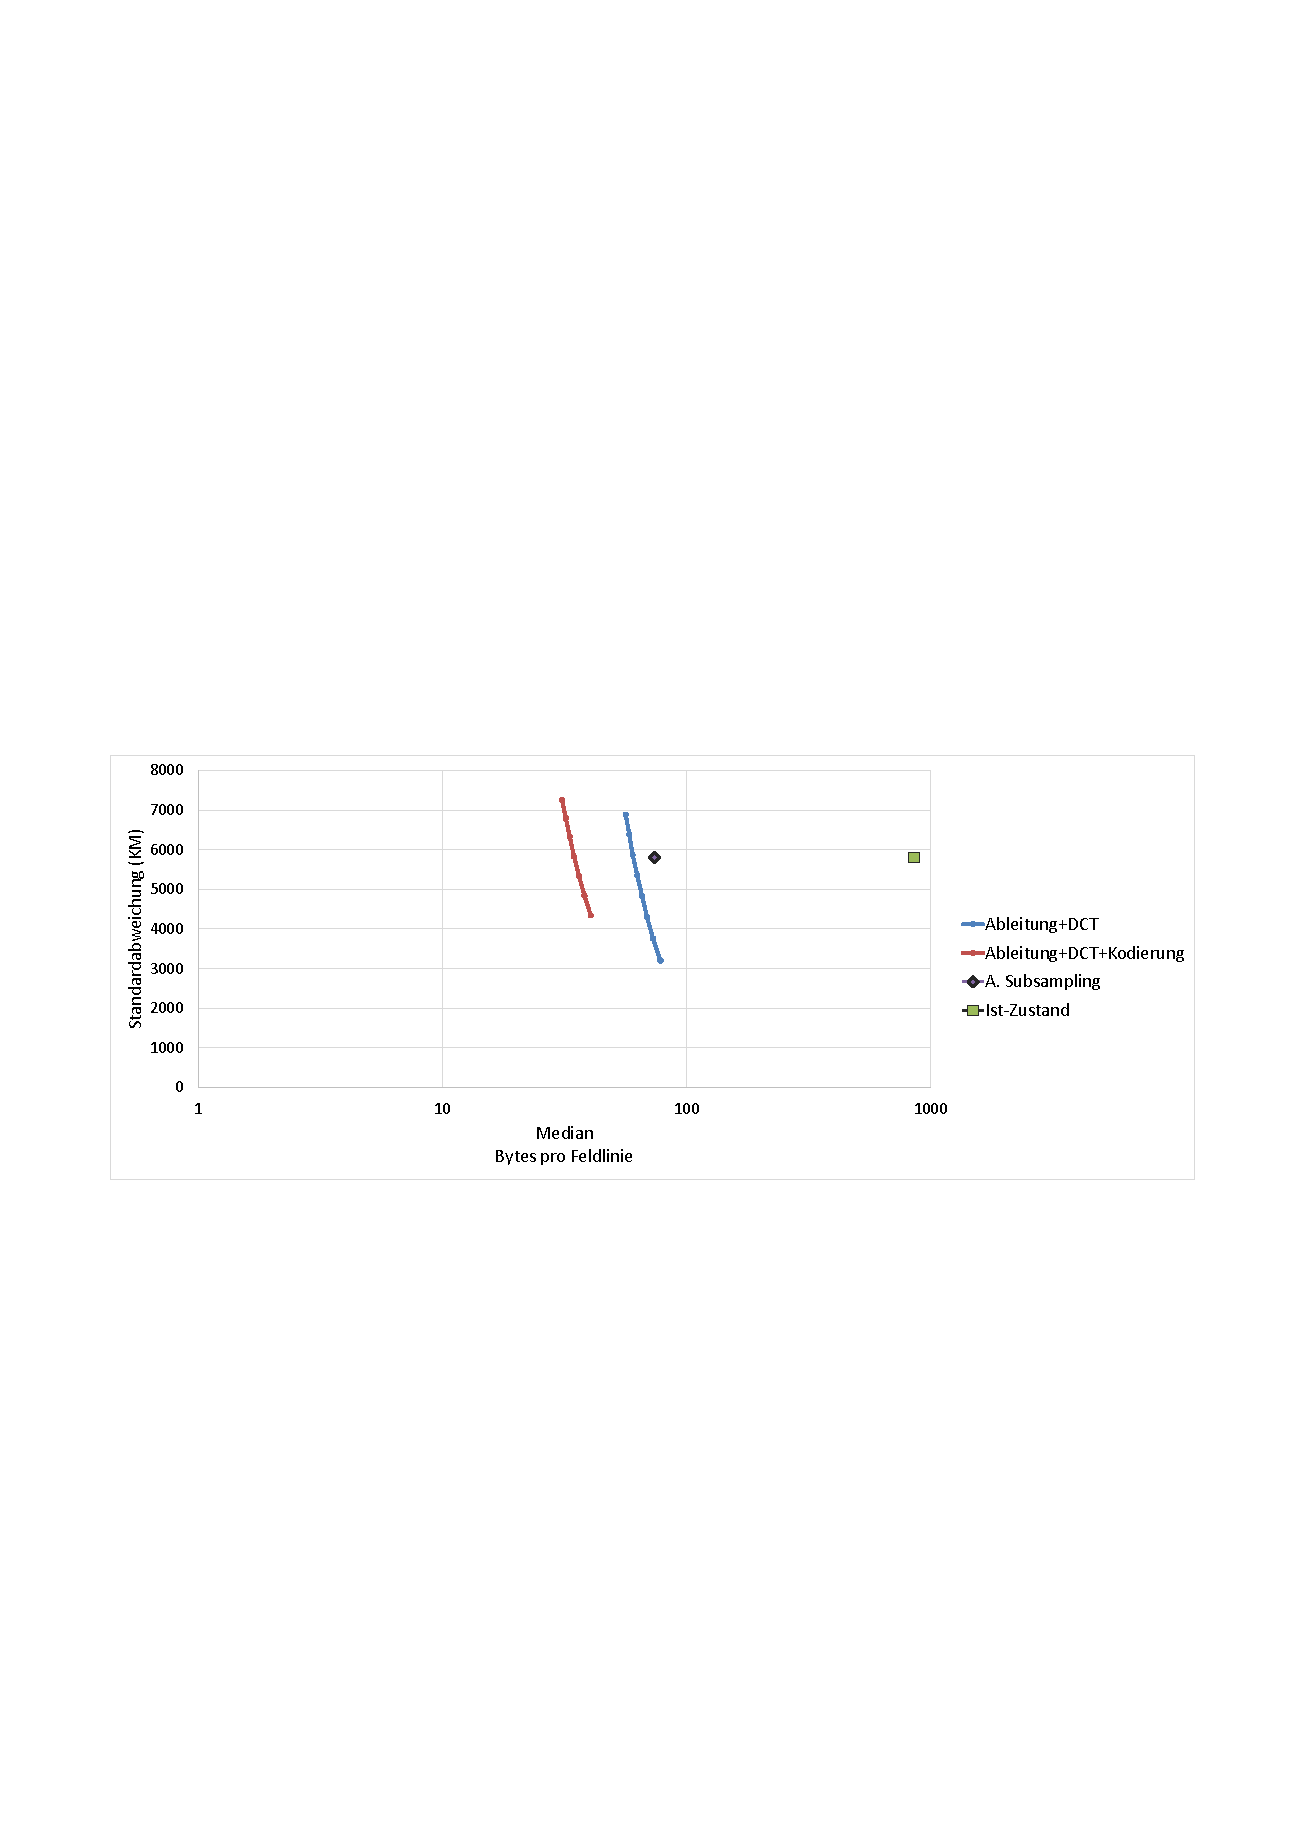
\includegraphics[trim = 1.8cm 11.25cm 1.8cm 12.75cm, clip=true,width=1\textwidth,keepaspectratio]{./pictures/resultate/loesung1/loesung1-6/loesung1_6.pdf}
	\caption{Vergleich der Kompression mit und ohne Kodierung}
	\label{resultate:loesung1:dct:kodierung}
\end{figure}
Das Diagramm der Abbildung \ref{resultate:loesung1:dct:kodierung} zeigt den Einfluss der Kodierung auf die Kompressionsrate. Es bewirkt eine deutliche Verbesserung gegenüber der vorhergehenden Variante, ohne die Qualität der Kompression negativ zu beeinflussen. Bei einer Vergleichbaren Genauigkeit wie die Ist-Kompression weist diese Variante eine Kompressionsrate von 24.5 auf.

\subsubsection{Variante: Randbehandlung+DCT+Kodierung} \label{resultate:loesung1:dct:randbeh+byte}
Bei dieser Variante wird mit zusätzlichen Daten am Anfang und am Ende der Feldlinie die Artefakte aus Abschnitt \ref{resultate:dct} behoben. Die zusätzlichen Daten lassen die Feldlinie abflachen. Es wird erforscht, ob diese Darstellung der Feldlinien eine bessere Kompressionsrate zur ähnlichen Abweichung erlaubt. 

\begin{figure}[!htbp]
	\center	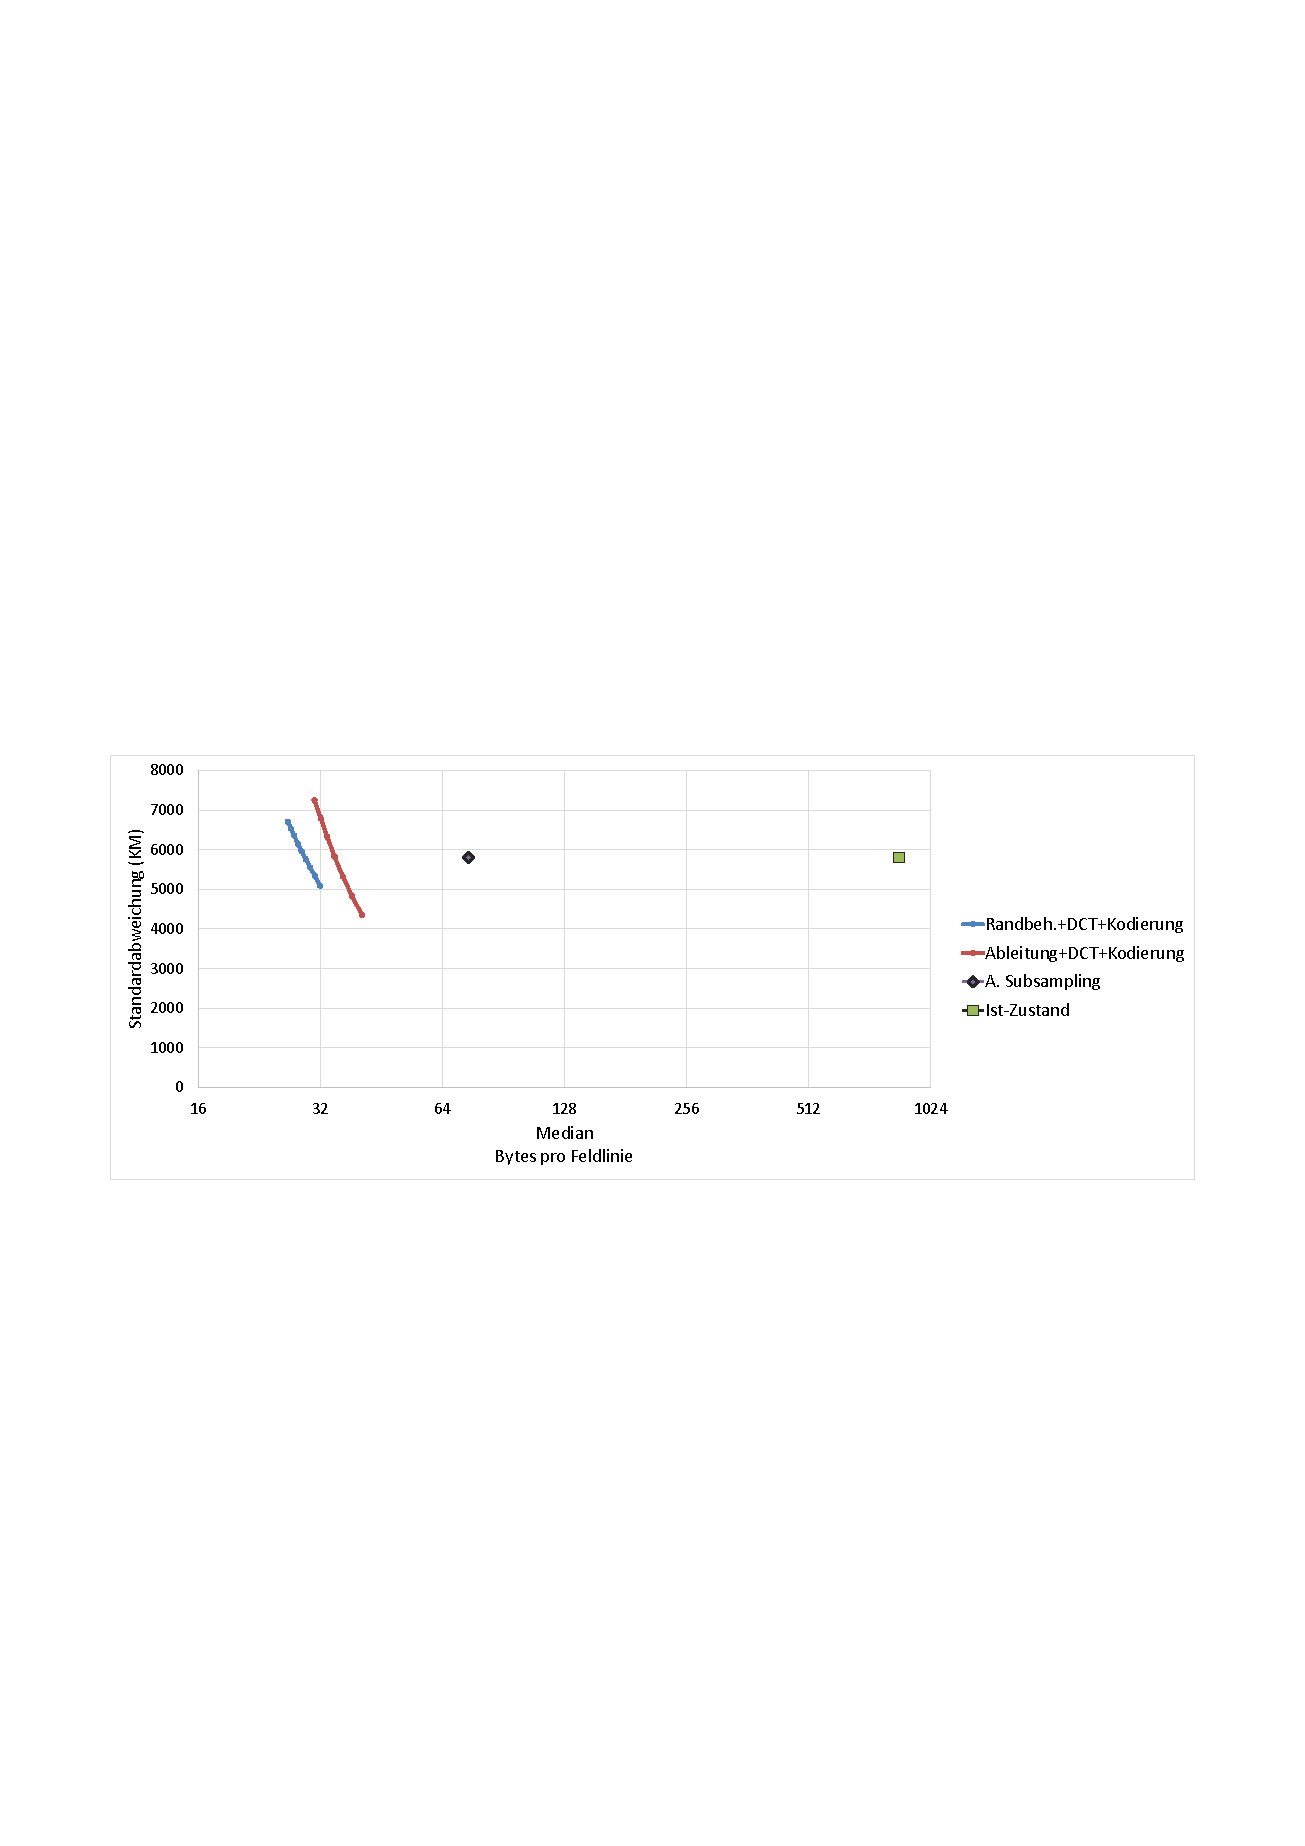
\includegraphics[trim = 1.8cm 11.25cm 1.8cm 12.75cm, clip=true,width=1\textwidth,keepaspectratio]{./pictures/resultate/loesung1/loesung1-7/loesung1_7.pdf}
	\caption{Vergleich des Einflusses der Randbehandlung}
	\label{resultate:loesung1:dct:randbehandlung}
\end{figure}
Das Diagramm der Abbildung \ref{resultate:loesung1:dct:randbehandlung} zeigt den Vergleich der Variante mit Randbehandlung und der vorgehenden Variante, welche die Feldlinie ableitet. Die zusätzlichen Daten erlauben eine höhere Kompressionsrate zu einer ähnlichen Abweichung.\\
Diese Variante führt Artefakte ein, welche in der Standardabweichung nicht ins Gewicht fallen. Im folgenden Abschnitt \ref{resultate:loesung1:ringing} werden diese Artefakte besprochen.

\subsubsection{Ringing-Artefakte}\label{resultate:loesung1:ringing}
Obwhol die Variante aus Abschnitt \ref{resultate:loesung1:dct:randbeh+byte} eine vergleichbare Standardabweichung aufweist, wie die Ist-Kompression, sind auf der JHelioviewer Visualisierung deutliche Artefakte zu sehen. Die Abbildung \ref{resultate:loesung1:dct:randbehandlung:jvhartefakte} vergleicht die originalen mit dekomprimierten Feldlinien. Die Artefakte äussern sich als Oszillationen in den dekomprimierten Feldlinien.

\begin{figure}[!htbp]
	\center
	\frame{
	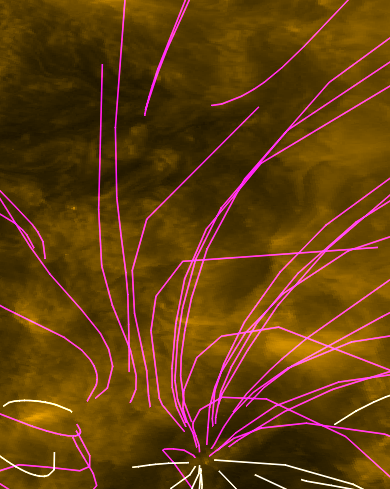
\includegraphics[width=0.8\textwidth,height=6cm,keepaspectratio]{./pictures/resultate/loesung1/ringing/actual.png}}
		\frame{
	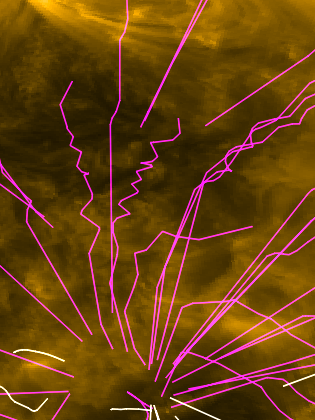
\includegraphics[width=0.8\textwidth,height=6cm,keepaspectratio]{./pictures/resultate/loesung1/ringing/sol7.png}}
	\caption{Artefakte der Kompression. Links sind die originalen Feldlinien, rechts die Dekomprimierten.}
	\label{resultate:loesung1:dct:randbehandlung:jvhartefakte}
\end{figure} 
In diesem Fall scheint die Standardabweichung als Fehlermass zu versagen: Da die Oszillationen nahe an der originalen Feldlinie liegen, bleiben die Abweichung klein. Jedoch sind die Artefakte für das menschliche Auge inakzeptabel.\\
Interessant ist, dass die abgeleiteten Feldlinien aus Abschnitt \ref{resultate:loesung1:ableitung_dct_kodierung} ähnliche Artefakte aufweisen, jedoch sind sie weniger ausgeprägt. Die Ableitung scheint die Artefakte zu dämpfen. Die Abbildung \ref{resultate:loesung1:dct:randbehandlung:jvhartefakte_loesung6} zeigt die Artefakte der abgeleiteten Feldlinien.

\begin{figure}[!htbp]
	\center
	\frame{
	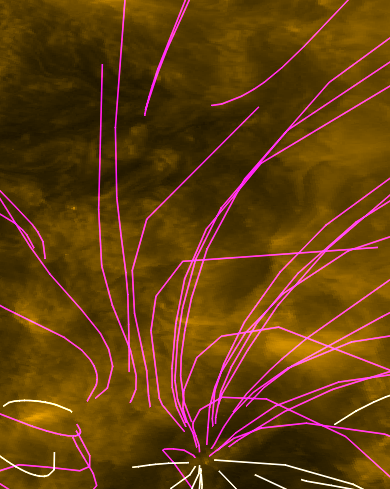
\includegraphics[width=0.8\textwidth,height=6cm,keepaspectratio]{./pictures/resultate/loesung1/ringing/actual.png}}
		\frame{
	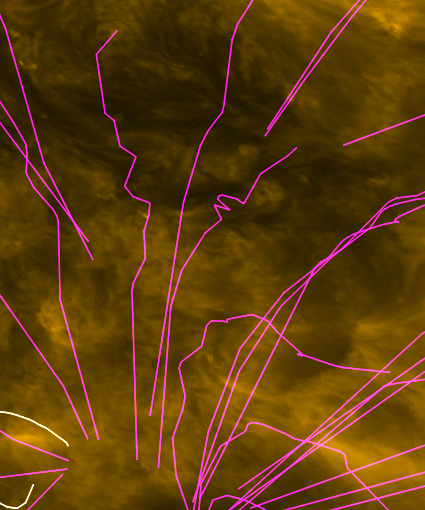
\includegraphics[width=0.8\textwidth,height=6cm,keepaspectratio]{./pictures/resultate/loesung1/ringing/sol6.png}}
	\caption{Artefakte der Kompression, links sind die originalen Feldlinien, rechts die Dekomprimierten der Variante \ref{resultate:loesung1:ableitung_dct_kodierung}.}
	\label{resultate:loesung1:dct:randbehandlung:jvhartefakte_loesung6}
\end{figure}
Die oszillierenden Artefakte sind typisch für eine Datenkompression mit einer Diskreten Kosinus Transformation und sind als Ringing-Artefakte \cite{wiki:ringing:artefacts} bekannt. Sie treten ebenfalls bei JPEG/JFIF oder MP3 Kompressionen auf: Abrupte Steigungen im Inputsignal werden in der DCT durch hochfrequente Anteile dargestellt. Durch die Quantisierung der hochfrequenten Anteile werden oszillierende Artefakte eingefügt.\\
Die Feldlinien, welche am stärksten von den Artefakten betroffen sind, sind die ''Weltall zur Sonne'' oder ''Sonne ins Weltall'' Feldlinien. Sie verhalten sich nicht wie harmonische Halbwellen sondern steigen oft monoton, mit teils abrupten Richtungswechseln in der Nähe der Sonnenoberfläche. Die Abbildung \ref{resultate:loesung1:dct:randbehandlung:harte_richtungswechsel} zeigt ein Beispiel solcher Feldlinien. Die abrupten Wechsel führen zu abrupten Steigungen in den einzelnen Kanälen.

\begin{figure}[!htbp]
\center
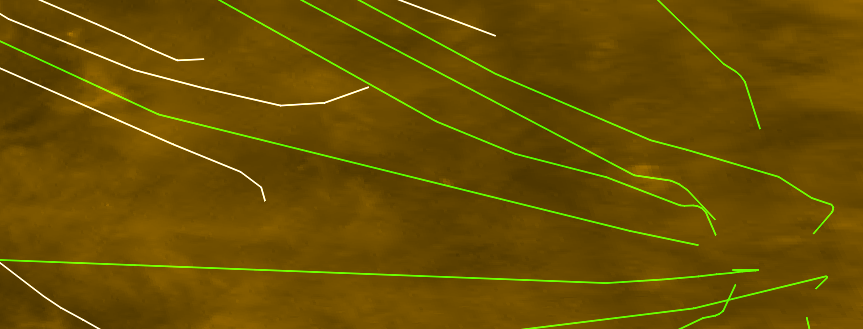
\includegraphics[width=0.4\textwidth,height=6cm,keepaspectratio]{./pictures/resultate/loesung1/ringing/haar-like.png}
	\caption{Abrupte Steigungen bei Feldlinien, welche von der Sonne ins Weltall führen.}
	\label{resultate:loesung1:dct:randbehandlung:harte_richtungswechsel}
\end{figure}

\subsubsection{Behandlung der Ringing-Artefakte} \label{resultate:loesung1:behandlung_ringing}
Um eine optimale Kompression der Feldlinien zu erreichen, müssen die Ringing-Artefakte behandelt werden. Im Abschnitt \ref{resultate:loesung1:ringing} wurde erwähnt, dass nicht alle Varianten gleich ausgeprägte Artefakte verursachen. Es wurde ebenfalls besprochen, dass die Feldlinien, welche von der Sonnenoberfläche zu Oberfläche führen, weniger ausgeprägte Artefakte mit sich bringen. In diesem Abschnitt wird erforscht, welche Variante die ''Sonne zu Sonne'' und welche die ''Weltall zur Sonne'' oder ''Sonne ins Weltall'' Feldlinien optimal approximieren kann, ohne zusätzliche Ringing-Artefakte hinzuzufügen. Für die Messung der Artefakte wird die PSNR-HVS-M Metrik aus Abschnitt \ref{testsetup:psnr} verwendet.\\
Für den Test werden insgesamt vier Varianten verglichen. Die Variante der abgeleiteten Feldlinien aus Abschnitt \ref{resultate:loesung1:ableitung_dct_kodierung} und die Variante der Randbehandlung aus Abschnitt \ref{resultate:loesung1:dct:randbeh+byte}. Die Varianten werden jeweils mit und ohne PCA gemessen. Die PCA wird hier nochmals überprüft, da sie die Ringing-Artefakte auf einen Kanal beschränken kann.

\begin{figure}[!htbp]
	\center	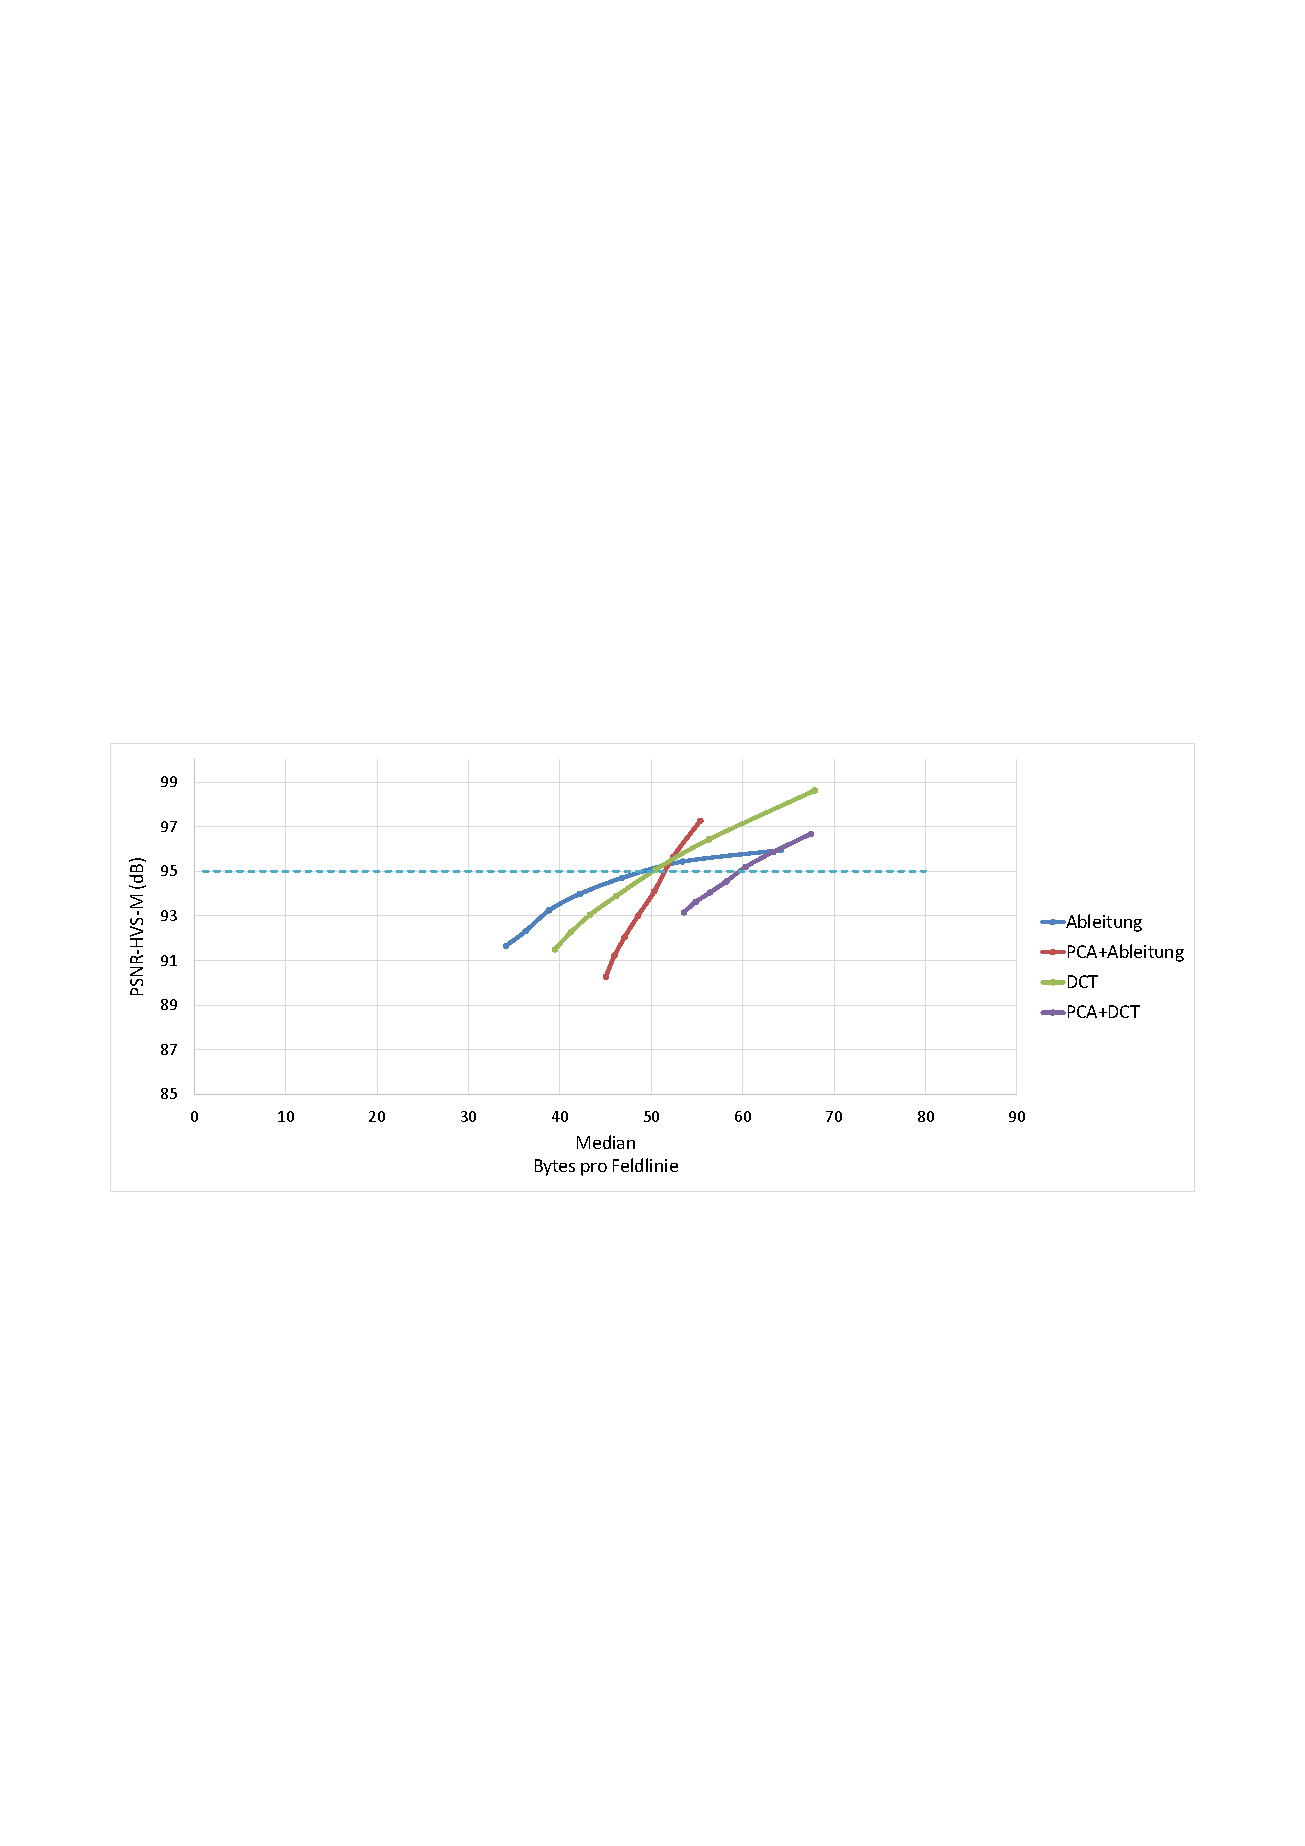
\includegraphics[trim = 1.8cm 11cm 1.8cm 12.5cm, clip=true,width=1\textwidth,keepaspectratio]{./pictures/resultate/loesung1/ringing/sts.pdf}
	\caption{Approximation der Feldlinien ''Sonnenoberfläche zu Sonnenoberfläche''. Je höher die PSNR-HVS-M, desto besser ist die Approximation. }	\label{resultate:loesung1:dct:behandlung_ringing:sts}
\end{figure} 
\begin{figure}[!htbp]
	\center
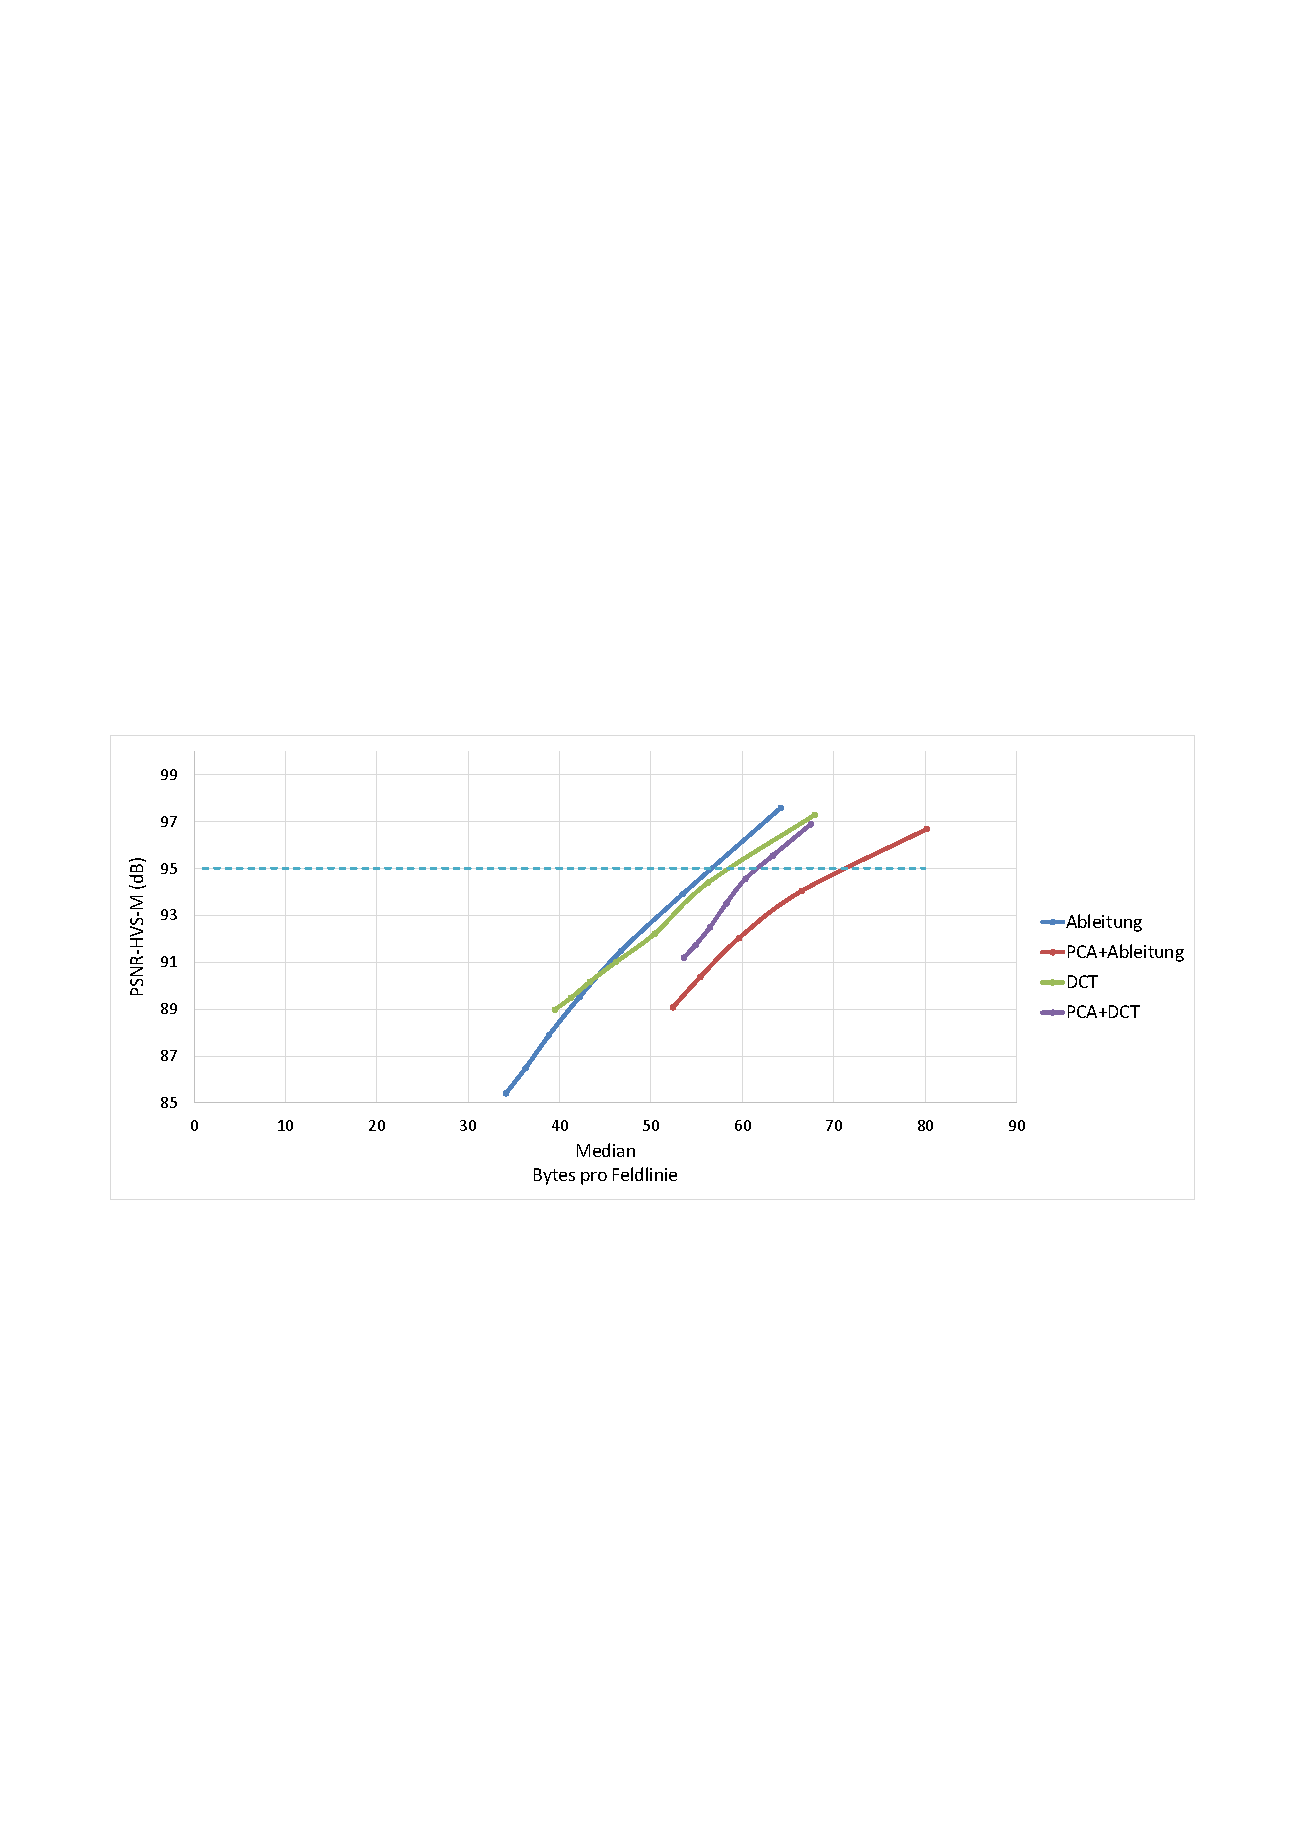
\includegraphics[trim = 1.8cm 11cm 1.8cm 12.4cm, clip=true,width=1\textwidth,keepaspectratio]{./pictures/resultate/loesung1/ringing/nosts.pdf}
	\caption{Approximation der der Feldlinien ''Sonnenoberfläche ins Weltall'' oder ''Weltall zur Sonnenoberfläche''. Je höher die PSNR-HVS-M, desto besser ist die Approximation.}	\label{resultate:loesung1:dct:behandlung_ringing:nosts}
\end{figure}
Das Diagramm der Abbildung \ref{resultate:loesung1:dct:behandlung_ringing:sts} zeigt die Resultate der unterschiedlichen Varianten bei den Feldlinien ''Sonnenoberfläche zur Sonnenoberfläche''. Bei einer PSNR-HVS-M von über 95 dB sind die Artefakte genügend schwach ausgeprägt, sodass das menschliche Auge sie nicht mehr erkennen kann. Interessant ist, dass drei Varianten ähnlich viel Speicherplatz benötigen, für eine artefaktfreie Approximation. Bei stärkerer Quantisierung treten bei den abgeleiteten Feldlinien deutlich weniger Artefakte auf. Dies deckt sich mit der Beobachtung aus dem Abschnitt \ref{resultate:loesung1:ringing}.\\
Ebenfalls interessant ist die Variante der PCA Transformation zusammen mit der Ableitung: Diese benötigt für eine beinahe artefaktfreie Approximation am wenigsten Speicherplatz, führt aber bei stärkerer Quantisierung viele Artefakte ein.

Das Diagramm der Abbildung  \ref{resultate:loesung1:dct:behandlung_ringing:nosts} zeigt, wie gut die Varianten die Feldlinien ''Sonne ins Weltall'' und ''Weltall zur Sonne'' approximieren können. Bei diesen Typen von Feldlinien dämpft die Ableitung ebenfalls die Artefakte. Jedoch weniger deutlich als bei den ''Sonne zur Sonne'' Feldlinien. Die PCA konnte auch bei diesen Typen von Feldlinien keinen messbaren Vorteil erbringen. Die zusätzlichen Parameter der PCA verbrauchen mehr Speicherplatz als durch die Transformation gewonnen werden.\\
Die DCT Variante aus Abschnitt \ref{resultate:loesung1:dct:randbeh+byte} fällt ab einer PSNR-HVS-M von 90 dB weniger schnell ab als die abgeleiteten Feldlinien. Bei diesem PSNR-HVS-M Wert sind aber die Artefakte bereits zu deutlich und nicht mehr akzeptabel. Aufgrund dieser Resultate wurde die Variante der abgeleiteten Feldlinien von Abschnitt \ref{resultate:loesung1:ableitung_dct_kodierung} ausgewählt. 

\subsubsection{Abschliessende Variante}
Für den abschliessenden Test wurde die Variante der abgeleiteten Feldlinien aus Abschnitt \ref{resultate:loesung1:ableitung_dct_kodierung} ausgewählt. Durch die Ableitung können die Ringing-Artefakte gedämpft werden. Die Quantisierung wurde angepasst, sodass die Feldlinien vom Typ ''Sonne zu Sonne'' stärker quantisiert werden, als die anderen Feldlinien. Durch diese Massnahme wird eine hohe Kompressionsrate erreicht ohne starke Ringing-Artefakte mit sich zu ziehen.

\begin{figure}[!htbp]
	\center	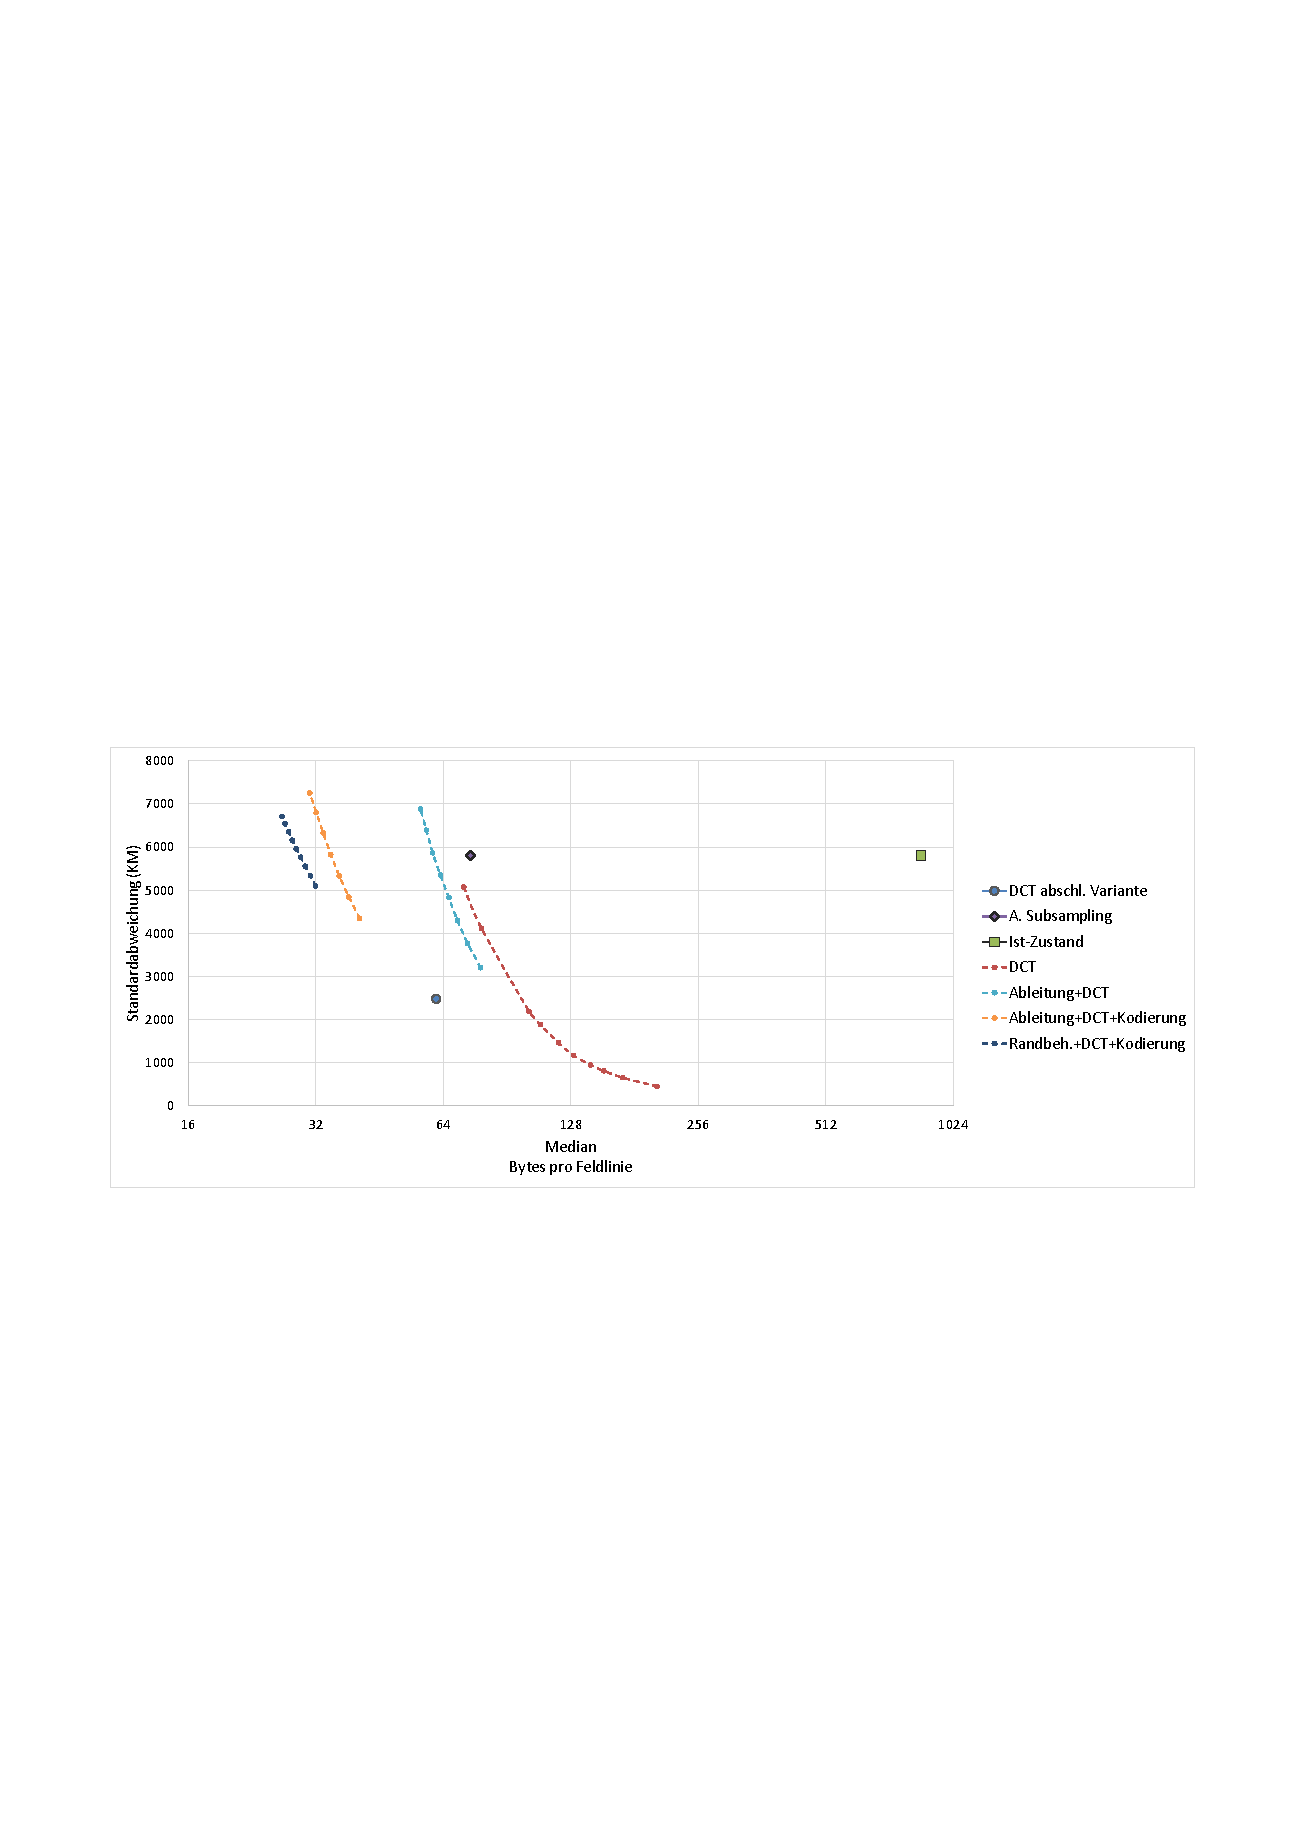
\includegraphics[trim = 1.8cm 11cm 1.8cm 12.5cm, clip=true,width=1\textwidth,keepaspectratio]{./pictures/resultate/loesung1/loesung1-12/resultate.pdf}
	\caption{Standardabweichung der abschliessenden DCT Variante.}	\label{resultate:loesung1:dct:abschliessend:standardabweichung}
\end{figure} 
Das Diagramm der Abbildung \ref{resultate:loesung1:dct:abschliessend:standardabweichung} zeigt die Standardabweichung der abschliessenden DCT Variante. Sie erreicht eine höhere Kompression als das Verfahren des Adaptiven Subsamplings und kann die Feldlinie zu einer tieferen Standardabweichung approximieren. Es wurde eine durchschnittliche Kompressionsrate von 14.1 erreicht, obwohl eine höhere Anzahl an Werte übertragen wird. Die Problematik dieses Verfahrens liegt darin, dass die DCT Kompression Ringing-Artefakte hinzufügt.\\
Durch die unterschiedliche Quantisierungen konnten die Ringing-Artefakte in Grenzen gehalten werden und erreichen einen PSNR-HVS-M  Wert von 94.0. Die ''Sonne zu Sonne'' Feldlinien können deutlich besser approximiert werden als die anderen Feldlinien. Würde die Simulation nur aus diesen Feldlinien bestehen, könnte eine Kompressionsrate von 15 bis 18 erreicht werden zu einem ähnlichen PSNR-HVS-M Wert. Die Feldlinien ''Sonne ins Weltall'' und ''Weltall zur Sonne'' sind schwieriger mit einer DCT artefaktfrei zu approximieren.  Durch das Zoom Feature vom JHelioviewer ist der Benutzer in der Lage die Ringing-Artefakte zu finden, sobald sie existieren. Das Linke Bild der Abbildung \ref{resultate:loesung1:dct:final:artefakte} zeigt die Artefakte der Kompression. Die Artefakte sind aus der Simulation, welche die markantesten Ringing-Artefakte aufweist. Durch eine Kurvenglättung kann der JHelioviewer die Artefakte verschleiern. Die komprimierten Daten enthalten mehr Werte, als die JHelioviewer Visualisierung darstellen kann. Die zusätzlichen Werte werden zur Glättung der Feldlinie verwendet. Den Effekt der Glättung ist in der Abbildung \ref{resultate:loesung1:dct:final:artefakte} abgebildet.

\begin{figure}[!htbp]
	\center
	\frame{
	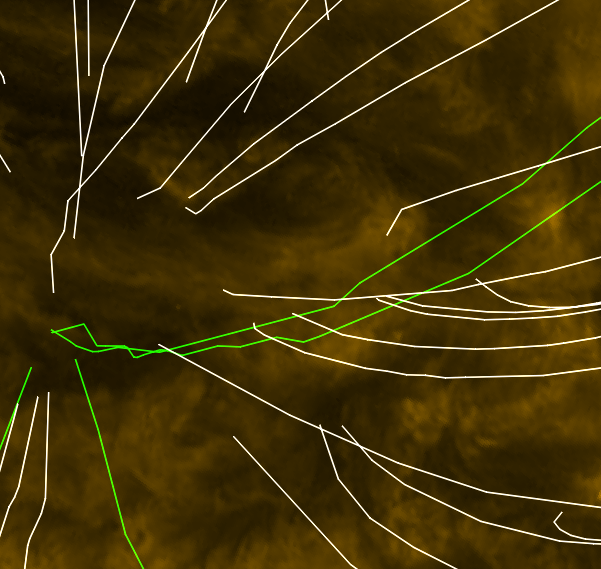
\includegraphics[width=0.8\textwidth,height=5cm,keepaspectratio]{./pictures/resultate/loesung1/loesung1-12/without_average_line.png}}
		\frame{
	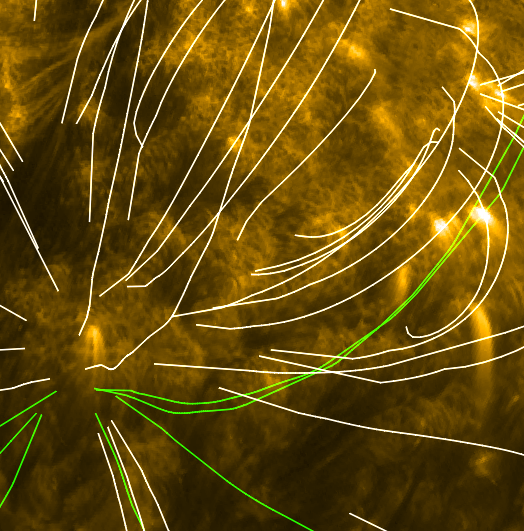
\includegraphics[width=0.8\textwidth,height=5cm,keepaspectratio]{./pictures/resultate/loesung1/loesung1-12/with_average_line.png}}
	\caption{Die am stärksten ausgeprägten Artefakte der abschliessenden Variante. Links ohne Glättung, rechts mit Glättung}
	\label{resultate:loesung1:dct:final:artefakte}
\end{figure}
Im Abschnitt \ref{konzept:loesung1} wurde erwähnt, dass Reduktion von Ringing-Artefakte ein aktives Forschungsfeld der Bildverarbeitung ist. Es existieren Post-Processing Filter, welche Ringing-Artefakte von dekomprimierten Bildern vermindern. Eine Möglichkeit die Kompression zu verbessern ist es, einen Post-Processing Filter für wissenschaftliche Daten zu entwickeln. Eine weitere Möglichkeit ist die Diskrete Kosinus Transformation durch eine Wavelet Transformation zu ersetzen. Diese ist weniger anfällig auf Ringing-Artefakte und hat das Potential eine ähnlich gute Kompression zu erreichen.

Beim Caching von 1000 Simulationen benötigt dieser Ansatz 70 Megabyte Arbeitsspeicher, etwa 15 Megabyte weniger als das Verfahren des Adaptiven Subsamplings. Wenn von derselben 5 Megabit Internenetverbindung ausgegangen wird, werden 112 Sekunden benötigt um 1000 Simulationen herunterzuladen. Pro Sekunde werden 9 Simulationen pro Sekunde übertragen. Der Durchsatzt konnte im Vergleich zum Verfahren mittels Adaptivem Subsampling um 2 Simulationen erhöht werden.

Die höhere Kompressionsrate führt zu einer höheren Komplexität der Dekompression. Die Laufzeit der Dekompression hängt im Wesentlichen von der Implementation der inversen DCT ab. Eine naive Implementation braucht für eine Dekompression etwa drei Sekunden (siehe Abschnitt \ref{anhang:performance}). Die meiste Zeit wird in der Berechnung der Kosinus-Werte verbraucht. Bei der DCT Implementation in dieser Arbeit werden die Kosinus-Werte über SoftReferences gecached. Der Cache passt sich somit an den Arbeitsspeicher an. Wie schnell die Dekompression ist, hängt hauptsächlich vom verfügbaren Arbeitsspeicher ab. Im besten Fall ergibt das eine Laufzeit von 65 Millisekunden und im Schlechtesten 350 Millisekunden. Mit einer Java Implementation der Fast-Cosine-Transform wird eine Laufzeit von 100 bis 135 Millisekunden erreicht. Im besten Fall ist die Implementation für diese Arbeit schneller, da es die Eigenschaft der Quantisierung ausnutzen kann: Es werden pro Feldlinie maximal 50 Koeffizienten übertragen. Die Komplexität kann dadurch auf $O(n*m)$ beschränkt werden, wobei $m$ die Anzahl der Koeffizienten ist. Die FDCT weist eine Komplexität von $O(n log(n))$ auf. Die Implementation verliert Laufzeit gegenüber der FDCT, wenn die Kosinus-Koeffizienten neu berechnet werden. Im Durchschnittsfall ist die FDCT Implementation schneller, was einen Durchsatz von 8 Simulationen pro Sekunde pro Thread führt.